\documentclass[12pt,a4paper]{article}
\usepackage[UTF8]{ctex}
\usepackage{amsmath}
\usepackage{amssymb}
\usepackage{amsthm}
\usepackage{graphicx}
\usepackage{hyperref}
\usepackage{geometry}
\usepackage{algorithm}
\usepackage{algorithmic}
\usepackage{listings}
\usepackage{xcolor}
\usepackage{fancyhdr}
\usepackage{booktabs}
\usepackage{tikz}
\usetikzlibrary{arrows,positioning,calc}
\usepackage{pgfplots}
\pgfplotsset{compat=1.18}
\geometry{left=2cm,right=2cm,top=2.5cm,bottom=2.5cm,headheight=15pt}
\setlength{\baselineskip}{1.1\baselineskip}
\setlength{\parskip}{0.5em}

% 导入通用样式
% 通用样式文件 - 统一所有文档的样式

% 目录样式设置 - 干净简洁,无边框,优化编号
% 使用基本 LaTeX 命令美化目录
\makeatletter
\renewcommand\@dotsep{2}
% 优化编号格式:减少缩进,使编号更紧凑
\renewcommand\l@section{\@dottedtocline{1}{0em}{1.2em}}
\renewcommand\l@subsection{\@dottedtocline{2}{1.2em}{1.8em}}
\renewcommand\l@subsubsection{\@dottedtocline{3}{3em}{2.2em}}
% 设置目录深度为3,显示到subsubsection级别
\setcounter{tocdepth}{3}
\makeatother

% 超链接设置 - 目录链接无颜色框
\hypersetup{
    colorlinks=true,
    linkcolor=black,          % 目录链接为黑色
    filecolor=black,
    urlcolor=blue,
    citecolor=black,
    pdfstartview=FitH,
    pdfborder={0 0 0},        % 无边框
    linkbordercolor={0 0 0},  % 链接边框颜色为黑色(不可见)
    pdfborderstyle={/S/U},    % 无边框样式
}

% 页眉页脚设置(在文档中重新定义)
\usepackage{fancyhdr}
% 注意:每个文档需要在导入 common_style.tex 后设置自己的页眉页脚

% 章节格式 - 简洁美观(使用基本命令)
\makeatletter
\renewcommand\section{\@startsection {section}{1}{\z@}%
                                   {-3.5ex \@plus -1ex \@minus -.2ex}%
                                   {2.3ex \@plus.2ex}%
                                   {\normalfont\Large\bfseries}}
\renewcommand\subsection{\@startsection{subsection}{2}{\z@}%
                                     {-3.25ex\@plus -1ex \@minus -.2ex}%
                                     {1.5ex \@plus .2ex}%
                                     {\normalfont\large\bfseries}}
\renewcommand\subsubsection{\@startsection{subsubsection}{3}{\z@}%
                                     {-3.25ex\@plus -1ex \@minus -.2ex}%
                                     {1.5ex \@plus .2ex}%
                                     {\normalfont\normalsize\bfseries}}
\makeatother

% 代码样式设置 - 简洁干净,无背景色
\definecolor{codegray}{rgb}{0.5,0.5,0.5}
\definecolor{keywordblue}{rgb}{0,0,0.8}
\definecolor{stringred}{rgb}{0.3,0.3,0.3}
\definecolor{commentgreen}{rgb}{0,0.5,0}

\lstdefinestyle{pythonstyle}{
    language=Python,
    % 无背景色 - 使用白色背景,与文档背景一致
    commentstyle=\color{commentgreen},      % 注释不用斜体
    keywordstyle=\color{keywordblue}\bfseries,
    stringstyle=\color{stringred},
    basicstyle=\ttfamily\small,
    breakatwhitespace=false,
    breaklines=true,
    captionpos=b,
    keepspaces=true,
    numbers=none,                           % 不显示行号
    showspaces=false,
    showstringspaces=false,
    showtabs=false,
    tabsize=4,
    frame=single,                          % 保留边框,但更简洁
    rulecolor=\color{black},
    framerule=0.5pt,                       % 细边框
    framexleftmargin=8pt,                  % 左边距(代码与左边框的距离)
    framexrightmargin=8pt,                 % 右边距(代码与右边框的距离)
    framextopmargin=6pt,                   % 上边距(代码与上边框的距离)
    framexbottommargin=6pt,                % 下边距(代码与下边框的距离)
    morekeywords={import,from,as,class,def,return,yield,lambda,if,elif,else,for,while,break,continue,pass,try,except,finally,raise,assert,with,del,global,nonlocal,and,or,not,in,is},
    identifierstyle=\color{black},
}

\lstset{style=pythonstyle}

% 封面宏定义
\newcommand{\makecover}[5]{%
    \newpage
    \thispagestyle{empty}
    \vspace*{1.5cm}
    \begin{center}
        \vspace{2cm}
        {\fontsize{48}{58}\selectfont\bfseries #1}\\[0.8cm]
        \vspace{1.5cm}
        {\Large #2}\\[0.4cm]
        \vspace{1.5cm}
        {\large #3}\\[1.5cm]
        
        % 神经网络图 - 紧凑版本,无标签
        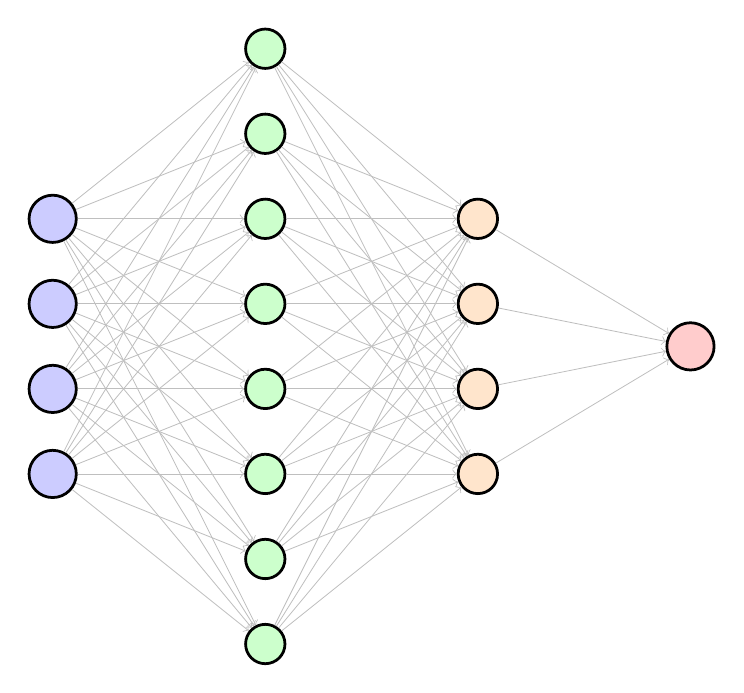
\begin{tikzpicture}[scale=0.9]
        % 定义神经元间距
        \def\spacing{1.2}
        
        % 输入层 - 4个神经元,关于横轴对称
        \node[circle, draw, minimum size=0.6cm, fill=blue!20, line width=1pt] (x1) at (0, -1.8) {};
        \node[circle, draw, minimum size=0.6cm, fill=blue!20, line width=1pt] (x2) at (0, -0.6) {};
        \node[circle, draw, minimum size=0.6cm, fill=blue!20, line width=1pt] (x3) at (0, 0.6) {};
        \node[circle, draw, minimum size=0.6cm, fill=blue!20, line width=1pt] (x4) at (0, 1.8) {};
        
        % 隐藏层1 - 8个神经元,关于横轴对称
        \node[circle, draw, minimum size=0.5cm, fill=green!20, line width=1pt] (h11) at (3, -4.2) {};
        \node[circle, draw, minimum size=0.5cm, fill=green!20, line width=1pt] (h12) at (3, -3.0) {};
        \node[circle, draw, minimum size=0.5cm, fill=green!20, line width=1pt] (h13) at (3, -1.8) {};
        \node[circle, draw, minimum size=0.5cm, fill=green!20, line width=1pt] (h14) at (3, -0.6) {};
        \node[circle, draw, minimum size=0.5cm, fill=green!20, line width=1pt] (h15) at (3, 0.6) {};
        \node[circle, draw, minimum size=0.5cm, fill=green!20, line width=1pt] (h16) at (3, 1.8) {};
        \node[circle, draw, minimum size=0.5cm, fill=green!20, line width=1pt] (h17) at (3, 3.0) {};
        \node[circle, draw, minimum size=0.5cm, fill=green!20, line width=1pt] (h18) at (3, 4.2) {};
        
        % 隐藏层2 - 4个神经元,关于横轴对称
        \node[circle, draw, minimum size=0.5cm, fill=orange!20, line width=1pt] (h21) at (6, -1.8) {};
        \node[circle, draw, minimum size=0.5cm, fill=orange!20, line width=1pt] (h22) at (6, -0.6) {};
        \node[circle, draw, minimum size=0.5cm, fill=orange!20, line width=1pt] (h23) at (6, 0.6) {};
        \node[circle, draw, minimum size=0.5cm, fill=orange!20, line width=1pt] (h24) at (6, 1.8) {};
        
        % 输出层 - 1个神经元,在横轴上
        \node[circle, draw, minimum size=0.6cm, fill=red!20, line width=1pt] (y) at (9, 0) {};
        
        % 输入层到隐藏层1的连接
        \foreach \i in {1,...,4}
            \foreach \j in {1,...,8}
                \draw[->, gray!50, line width=0.3pt] (x\i) -- (h1\j);
        
        % 隐藏层1到隐藏层2的连接
        \foreach \i in {1,...,8}
            \foreach \j in {1,...,4}
                \draw[->, gray!50, line width=0.3pt] (h1\i) -- (h2\j);
        
        % 隐藏层2到输出层的连接
        \foreach \i in {1,...,4}
            \draw[->, gray!50, line width=0.3pt] (h2\i) -- (y);
        \end{tikzpicture}
        
        \vfill
        \vspace{2cm}
        {\normalsize #5}
        \vspace{1.5cm}
    \end{center}
    \newpage
}



% 页眉页脚设置
\pagestyle{fancy}
\fancyhf{}
\fancyhead[L]{\leftmark}
\fancyhead[R]{\thepage}
\fancyfoot[C]{\small 深度学习核心理论与技术}
\renewcommand{\headrulewidth}{0.3pt}
\renewcommand{\footrulewidth}{0.3pt}

\title{深度学习核心理论与技术}
\author{}
\date{\today}

\newtheorem{definition}{定义}[section]
\newtheorem{theorem}{定理}[section]
\newtheorem{example}{例}[section]
\newtheorem{remark}{注}[section]

\begin{document}

% 封面
\makecover{深度学习核心理论与技术}{神经网络 · CNN · RNN · Transformer · 优化技术}{深入理解深度学习的核心原理与实践应用}{AI/ML 系列教程}

\maketitle

\tableofcontents
\newpage

\part{第一部分:神经网络基础}

\section{引言}

深度学习(Deep Learning)是机器学习的一个子领域,通过构建具有多个隐藏层的神经网络来学习数据的层次化表示。深度学习在计算机视觉、自然语言处理、语音识别、游戏AI等领域取得了突破性进展,成为当前人工智能领域最活跃的研究方向之一。

\textbf{深度学习的核心优势}:
\begin{itemize}
    \item \textbf{自动特征提取}:无需人工设计特征,网络能够自动学习数据的层次化特征表示
    \item \textbf{处理复杂非线性关系}:通过多层非线性变换,能够建模高度复杂的函数关系
    \item \textbf{端到端学习}:直接从原始输入学习到最终输出,减少中间环节的信息损失
    \item \textbf{强大的表示能力}:深度网络具有强大的函数逼近能力,能够学习任意复杂的映射关系
    \item \textbf{迁移学习能力}:预训练模型可以迁移到相关任务,提高学习效率
\end{itemize}

\textbf{深度学习面临的挑战}:
\begin{itemize}
    \item \textbf{数据需求量大}:通常需要大量标注数据才能训练出有效的模型
    \item \textbf{计算资源消耗}:训练深度网络需要强大的计算资源(GPU/TPU)
    \item \textbf{可解释性不足}:深度网络的决策过程往往缺乏可解释性,难以理解其内部机制
    \item \textbf{过拟合风险}:模型容量大,容易在训练数据上过拟合
    \item \textbf{实时性要求}:某些应用场景对推理速度有严格要求
    \item \textbf{数据稀疏性}:在某些领域(如医疗、金融)高质量数据稀缺
\end{itemize}

本文档系统性地介绍深度学习的核心理论、主要架构和关键技术,涵盖神经网络基础、深度网络架构、优化技术、表示学习、注意力机制以及强化学习等内容。

\section{神经网络基础}

\subsection{感知机}

感知机(Perceptron)是最简单的神经网络模型,由 Frank Rosenblatt 于1957年提出,是神经网络和深度学习的起点。

\begin{definition}[感知机]
感知机是一个二分类线性分类模型,其输入为特征向量 $\mathbf{x} = [x_1, x_2, \ldots, x_n]^T$,输出为类别标签 $y \in \{-1, +1\}$。

感知机的数学表达式为:
\begin{equation}
f(\mathbf{x}) = \text{sign}(\mathbf{w}^T \mathbf{x} + b) = \begin{cases}
+1 & \text{if } \mathbf{w}^T \mathbf{x} + b \geq 0 \\
-1 & \text{if } \mathbf{w}^T \mathbf{x} + b < 0
\end{cases}
\end{equation}

其中,$\mathbf{w} = [w_1, w_2, \ldots, w_n]^T$ 是权重向量,$b$ 是偏置项。
\end{definition}

\textbf{感知机的几何解释}:感知机实际上是在特征空间中构造一个超平面 $\mathbf{w}^T \mathbf{x} + b = 0$,将数据分为两类。权重向量 $\mathbf{w}$ 垂直于超平面,指向正类区域。

\textbf{感知机学习算法}:使用错误驱动的学习规则,当分类错误时更新权重:

\begin{algorithm}
\caption{感知机学习算法}
\begin{algorithmic}[1]
\REQUIRE 训练数据集 $\{(\mathbf{x}_1, y_1), (\mathbf{x}_2, y_2), \ldots, (\mathbf{x}_m, y_m)\}$,学习率 $\eta$
\ENSURE 权重向量 $\mathbf{w}$ 和偏置 $b$
\STATE 初始化 $\mathbf{w} = \mathbf{0}$,$b = 0$
\REPEAT
    \FOR{每个样本 $(\mathbf{x}_i, y_i)$}
        \IF{$y_i(\mathbf{w}^T \mathbf{x}_i + b) \leq 0$}
            \STATE $\mathbf{w} \leftarrow \mathbf{w} + \eta y_i \mathbf{x}_i$
            \STATE $b \leftarrow b + \eta y_i$
        \ENDIF
    \ENDFOR
\UNTIL{没有分类错误}
\end{algorithmic}
\end{algorithm}

\textbf{感知机的局限性}:感知机只能解决线性可分问题。对于线性不可分问题(如异或问题),单层感知机无法解决,这促使了多层感知机的提出。

\subsection{多层感知机}

多层感知机(Multi-Layer Perceptron, MLP)通过引入隐藏层和激活函数,能够解决非线性分类问题。

\begin{definition}[多层感知机]
多层感知机是由多个全连接层组成的神经网络,每层包含多个神经元。一个 $L$ 层的 MLP 可以表示为:

\begin{align}
\mathbf{h}^{(0)} &= \mathbf{x} \\
\mathbf{h}^{(l)} &= \sigma(\mathbf{W}^{(l)} \mathbf{h}^{(l-1)} + \mathbf{b}^{(l)}), \quad l = 1, 2, \ldots, L-1 \\
\mathbf{y} &= \mathbf{W}^{(L)} \mathbf{h}^{(L-1)} + \mathbf{b}^{(L)}
\end{align}

其中,$\mathbf{W}^{(l)}$ 是第 $l$ 层的权重矩阵,$\mathbf{b}^{(l)}$ 是偏置向量,$\sigma$ 是激活函数。
\end{definition}

\subsubsection{隐藏层详解}

\textbf{概念解释}:隐藏层(Hidden Layer)是人工神经网络中的核心组成部分,位于输入层和输出层之间。之所以称为"隐藏",是因为这些层的输出不直接暴露给外部世界(不像输入层接收原始数据、输出层给出最终预测),而是用于内部特征表示的学习。

\textbf{数学表示}:

从数学和结构上看:
\begin{itemize}
    \item \textbf{输入层}:接收原始特征,记为 $\mathbf{x} \in \mathbb{R}^d$
    \item \textbf{隐藏层}:对输入进行非线性变换,提取更高层次的抽象特征。第 $l$ 层的输出为:
    \begin{equation}
    \mathbf{h}^{(l)} = \sigma\left( \mathbf{W}^{(l)} \mathbf{h}^{(l-1)} + \mathbf{b}^{(l)} \right)
    \end{equation}
    其中:
    \begin{itemize}
        \item $\mathbf{W}^{(l)}$ 是权重矩阵(可学习参数)
        \item $\mathbf{b}^{(l)}$ 是偏置向量
        \item $\sigma(\cdot)$ 是激活函数(如 ReLU、Sigmoid、Tanh)
        \item $\mathbf{h}^{(0)} = \mathbf{x}$
    \end{itemize}
    \item \textbf{输出层}:基于最后一层隐藏层的表示,生成最终预测
\end{itemize}

\textbf{关键作用}:隐藏层通过多层非线性组合,使网络能够拟合复杂的函数(如图像识别、自然语言理解等)。没有隐藏层(即只有输入→输出),网络就退化为线性模型,表达能力极其有限。

\textbf{配置隐藏层}:

当你在代码中配置隐藏层时,实际上在配置:

\begin{itemize}
    \item \textbf{神经元数量}:每层的神经元数量(即维度),也叫"隐藏单元数"或"宽度(width)"
    \item \textbf{权重矩阵形状}:如 $100 \times 256$ 表示输入100维,输出256维
    \item \textbf{激活函数}:指定该隐藏层使用的激活函数(如 ReLU)
    \item \textbf{层数}:决定了网络的深度(depth)
\end{itemize}

\textbf{示例}:

\begin{lstlisting}[caption=隐藏层配置示例]
# 配置示例:输入100维 → 隐藏层1: 256个神经元 → 隐藏层2: 128个神经元 → 输出1维
# 这实际上定义了:
# - 第1层:100 × 256 的权重矩阵,256个神经元
# - 第2层:256 × 128 的权重矩阵,128个神经元  
# - 输出层:128 × 1 的权重矩阵,1个神经元
\end{lstlisting}

\textbf{超参数影响}:
\begin{itemize}
    \item 神经元越多、层数越深 → 模型越复杂,拟合能力越强,但也更容易过拟合
    \item 在深度学习中,常用 2~4 层 MLP,每层 128~512 个神经元
\end{itemize}

\textbf{特征学习的层次性}:

每一个"隐藏层"其实就是一个向量空间变换器:把低层特征映射到高层语义特征。例如:
\begin{itemize}
    \item 第1层可能学到"边缘、线条"等低级特征
    \item 第2层可能学到"形状、纹理"等中级特征
    \item 第3层可能学到"物体部件"等高级特征
    \item 最终输出层预测"完整物体"的类别
\end{itemize}

\subsubsection{输入层、隐藏层、输出层的明确区分}

\textbf{核心定义}:

隐藏层(Hidden Layer)的定义是:既不是输入层,也不是输出层的所有中间层。

\begin{itemize}
    \item \textbf{输入层(Input Layer)}:负责接收原始数据(如特征向量、像素值等),不是隐藏层。
    \item \textbf{输出层(Output Layer)}:负责产生最终预测(如分类概率、回归值等),也不是隐藏层。
    \item \textbf{隐藏层}:只有夹在输入层和输出层之间的层才叫隐藏层。
\end{itemize}

\textbf{举例说明}:

对于一个3层网络(输入层 → 隐藏层 → 输出层),只有中间那层是隐藏层。如果网络有更多层,如输入层 → 隐藏层1 → 隐藏层2 → 输出层,那么隐藏层1和隐藏层2都是隐藏层。

\textbf{术语使用规范}:

\begin{itemize}
    \item \textbf{输入层}:不是隐藏层。无参数,仅传递数据。
    \item \textbf{中间层}:是隐藏层。如 \texttt{Linear(256,128) + ReLU},包含可学习参数。
    \item \textbf{输出层}:不是隐藏层。如 \texttt{Linear(128, 1)},用于最终映射。
\end{itemize}

\textbf{重要说明}:

虽然输出层通常是全连接层(用 Linear 实现,有权重和偏置),但我们不会称它为"隐藏层",因为它的功能是输出,不是隐藏表示。当说"模型有2个隐藏层"时,指的是中间有2个可学习的层,不包括输入和输出。

\subsubsection{编码(Encoding)与输入层的关系}

\textbf{核心概念区分}:

\begin{itemize}
    \item \textbf{编码(Encoding)}:将原始数据(如文本、类别、SQL语句、图像)转换为数值向量的过程。这是预处理步骤,发生在模型之外或模型最前端。
    \item \textbf{输入层(Input Layer)}:神经网络的第一层,接收已经编码好的数值向量作为输入。它本身不做编码,只是"起点"。
\end{itemize}

\textbf{数学表示}:

编码过程:$\mathbf{x} = \text{encode}(\text{原始输入})$,其中 $\mathbf{x} \in \mathbb{R}^d$ 是编码后的数值向量。

输入层:$\mathbf{h}^{(0)} = \mathbf{x}$,即输入层就是编码后的向量本身,不做任何变换。

\textbf{举例说明}:

\begin{example}[文本分类任务]
\begin{itemize}
    \item \textbf{原始输入}:文本"Hello World"
    \item \textbf{编码过程}:
    \begin{itemize}
        \item 分词:["Hello", "World"]
        \item 词嵌入(Embedding):将每个词转换为向量
        \item 结果:$\mathbf{x} \in \mathbb{R}^{d}$(如 $d=128$)
    \end{itemize}
    \item \textbf{输入层}:接收这个 $\mathbf{x}$ 向量,不做任何变换,直接传给第一个全连接层
\end{itemize}
\end{example}

\begin{example}[图像分类任务]
\begin{itemize}
    \item \textbf{原始输入}:一张 $28 \times 28$ 的图片(像素值 0~255)
    \item \textbf{编码过程}:
    \begin{itemize}
        \item 归一化到 $[0,1]$
        \item 展平成 $784$ 维向量
    \end{itemize}
    \item \textbf{输入层}:接收这 $784$ 维向量,直接送入第一个全连接层或卷积层
\end{itemize}
\end{example}

\textbf{关键结论}:

\begin{itemize}
    \item \textbf{"输入层就是做 encoding"}:不准确。输入层不执行 encoding,它只是接收已经编码好的数据。
    \item \textbf{"encoding 的结果作为输入层的值"}:正确。这是标准流程,编码后的向量 $\mathbf{x}$ 就是输入层的值。
    \item \textbf{"Embedding 层是输入层"}:不准确。\texttt{nn.Embedding} 是可学习的 encoding 模块,属于模型的第一层可学习模块,但它已经超出了"输入层"的范畴。
\end{itemize}

\textbf{代码示例}:

\begin{lstlisting}[caption=编码与输入层在代码中的体现]
import torch
import torch.nn as nn

# 假设原始输入是词索引: [2, 5, 1]
embedding = nn.Embedding(num_embeddings=1000, embedding_dim=64)  # 这是 encoding!
fc1 = nn.Linear(64, 128)  # 这才是真正的第一层(隐藏层)

x = torch.tensor([2, 5, 1])
emb = embedding(x)  # shape: (3, 64) ← encoded vector
out = fc1(emb)  # 输入给全连接层
\end{lstlisting}

\textbf{总结}:

输入层不等于编码,但输入层的值等于编码的结果。编码是数据预处理或模型前端的转换步骤,目的是把原始信息变成神经网络能处理的数值向量。输入层只是这个向量进入网络的入口,本身不做计算(无参数)。

更准确的说法是:"我们先把数据 encode 成向量,然后喂给神经网络的输入层。"

\subsubsection{输入层不做线性变换}

\textbf{核心结论}:

输入层本身不做任何线性变换(也不做非线性变换)。输入层只是一个"数据入口"或"占位符",它没有可学习的参数(如权重 $\mathbf{W}$ 和偏置 $\mathbf{b}$),也不执行任何计算(包括线性变换)。

\textbf{什么是线性变换}:

在线性代数和神经网络中,线性变换(更准确说是仿射变换)指:
\begin{equation}
\mathbf{z} = \mathbf{W} \mathbf{x} + \mathbf{b}
\end{equation}

其中:
\begin{itemize}
    \item $\mathbf{W}$:权重矩阵(可学习参数)
    \item $\mathbf{b}$:偏置向量(可学习参数)
\end{itemize}

这是全连接层(Linear/Dense Layer)的核心操作。只有包含可学习参数并执行上述运算的层,才做了线性变换。

\textbf{输入层的本质}:

输入层等于原始特征向量 $\mathbf{x}$ 本身。它的作用仅仅是将预处理或编码后的数据传递给网络的第一层可学习模块。

在数学上,输入层就是 $\mathbf{h}^{(0)} = \mathbf{x}$。没有 $\mathbf{W}$,没有 $\mathbf{b}$,没有运算。

\textbf{类比说明}:

输入层就像函数的参数,而不是函数体内的计算:

\begin{lstlisting}[caption=输入层与计算层的区别]
def neural_network(x):  # ← x 就是"输入层"
    z1 = W1 @ x + b1  # ← 第一个全连接层(才开始线性变换)
    a1 = relu(z1)
    ...
\end{lstlisting}

这里 $\mathbf{x}$ 本身不做任何事,只是被使用。

\textbf{常见误解澄清}:

\begin{itemize}
    \item \textbf{误解:"输入层是第一个 Linear 层"} \\
    \textbf{澄清}:错!第一个 \texttt{Linear} 层是第一个隐藏层(或输出层),不是输入层。输入层没有参数,而 \texttt{Linear} 层有可学习的权重和偏置。
    
    \item \textbf{误解:"输入层有神经元,所以会计算"} \\
    \textbf{澄清}:错!输入"神经元"只是对输入维度的形象说法(如"100维输入"说成"100个输入神经元"),但它们没有激活函数、没有权重,不进行计算。输入层只是数据的载体。
    
    \item \textbf{误解:"Embedding 是输入层"} \\
    \textbf{澄清}:不准确。\texttt{nn.Embedding} 是一个可学习的 encoding 层,属于模型的第一层可学习模块,但它已经超出了"输入层"的范畴。输入层是无参数的,而 \texttt{Embedding} 有可学习的参数。
\end{itemize}

\textbf{图示说明}:

\begin{center}
原始数据 $\to$ [Encoding] $\to$ $\mathbf{x} \in \mathbb{R}^{100}$(这就是输入层,无计算)\\
$\downarrow$\\
\texttt{[Linear($\mathbf{W}_1$, $\mathbf{b}_1$)]}(第一个全连接层,开始线性变换)\\
$\downarrow$\\
ReLU(...)
\end{center}

\textbf{特殊情况说明}:

在极少数文献或框架中,有人把标准化(Normalization)或固定投影放在最前面,例如:

\begin{lstlisting}[caption=标准化预处理]
x_norm = (x - mean) / std  # 数据标准化
z = W @ x_norm + b
\end{lstlisting}

但请注意:标准化是预处理,不属于网络参数。即使把它写进模型,也通常视为数据 pipeline 的一部分,而非"输入层的计算"。真正的"输入层"在理论和实践中都被定义为无参数、无变换的数据载体。

\textbf{总结}:

\begin{itemize}
    \item \textbf{输入层会做线性变换吗?} \\
    不会。输入层没有权重 $\mathbf{W}$ 和偏置 $\mathbf{b}$,不执行任何运算。
    
    \item \textbf{线性变换从哪开始?} \\
    从第一个全连接层(\texttt{Linear/Dense Layer})开始。这是网络中的第一个可学习模块。
    
    \item \textbf{输入层的作用是什么?} \\
    接收已编码的数值向量,作为网络计算的起点。它只是数据的入口,不做任何变换。
\end{itemize}

所以可以明确地说:"输入层只是数据的入口,真正的计算从第一层全连接层才开始。"

\subsection{激活函数详解}

激活函数(Activation Function)是神经网络中的关键组件,它引入非线性变换,使网络能够学习复杂的非线性函数关系。没有激活函数,多层神经网络就退化为单层线性模型。

\subsubsection{常用激活函数}

\textbf{1. Sigmoid 函数}

\textbf{数学公式}:
\begin{equation}
\sigma(x) = \frac{1}{1 + e^{-x}}
\end{equation}

\textbf{导数}:
\begin{equation}
\sigma'(x) = \sigma(x)(1 - \sigma(x))
\end{equation}

\textbf{输出范围}:$(0, 1)$

\textbf{用处}:
\begin{itemize}
    \item 二分类任务的输出层,输出概率
    \item 需要将输出映射到 $(0, 1)$ 区间的场景
    \item 门控机制(如 LSTM、GRU)
\end{itemize}

\textbf{为什么用 Sigmoid}:
\begin{itemize}
    \item \textbf{概率解释}:输出可以解释为概率,便于理解
    \item \textbf{平滑可导}:处处可导,梯度计算方便
    \item \textbf{历史原因}:早期神经网络常用,与生物神经元激活模式相似
\end{itemize}

\textbf{缺点}:
\begin{itemize}
    \item \textbf{梯度消失}:当输入很大或很小时,梯度接近0,导致深层网络难以训练
    \item \textbf{非零中心}:输出均值不为0,导致梯度更新效率低
    \item \textbf{计算成本}:涉及指数运算,计算较慢
\end{itemize}

\textbf{函数图像}:

\begin{center}
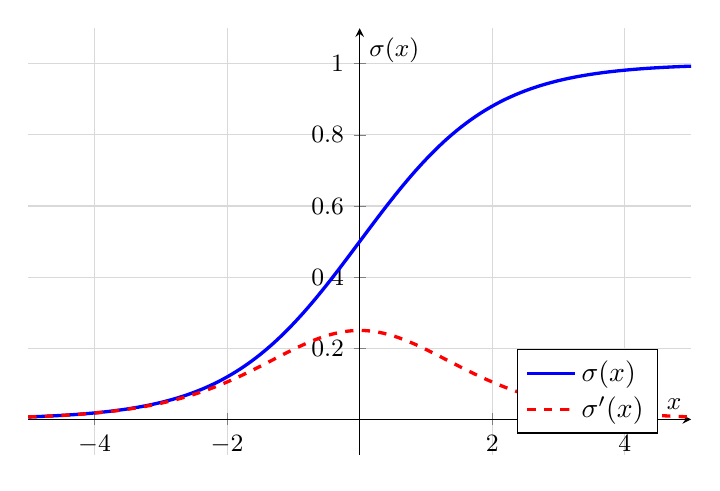
\begin{tikzpicture}
\begin{axis}[
    width=10cm,
    height=7cm,
    axis lines=middle,
    xlabel={$x$},
    ylabel={$\sigma(x)$},
    xmin=-5, xmax=5,
    ymin=-0.1, ymax=1.1,
    grid=major,
    grid style={gray!30},
    legend style={at={(0.95,0.05)},anchor=south east},
    legend cell align=left,
    smooth,
    samples=200,
    tick label style={font=\small},
    label style={font=\small},
]
\addplot[blue, very thick, domain=-5:5] {1/(1+exp(-x))};
\addplot[red, dashed, very thick, domain=-5:5] {1/(1+exp(-x))*(1-1/(1+exp(-x)))};
\legend{$\sigma(x)$, $\sigma'(x)$}
\end{axis}
\end{tikzpicture}
\end{center}

\textbf{2. Tanh 函数(双曲正切)}

\textbf{数学公式}:
\begin{equation}
\tanh(x) = \frac{e^x - e^{-x}}{e^x + e^{-x}} = \frac{2}{1 + e^{-2x}} - 1
\end{equation}

\textbf{导数}:
\begin{equation}
\tanh'(x) = 1 - \tanh^2(x)
\end{equation}

\textbf{输出范围}:$(-1, 1)$

\textbf{用处}:
\begin{itemize}
    \item RNN 中的隐藏层激活函数
    \item 需要零中心化输出的场景
    \item 数据归一化到 $(-1, 1)$ 区间
\end{itemize}

\textbf{为什么用 Tanh}:
\begin{itemize}
    \item \textbf{零中心化}:输出均值为0,梯度更新更高效
    \item \textbf{比 Sigmoid 更好}:在大多数情况下,tanh 比 sigmoid 表现更好
    \item \textbf{对称性}:关于原点对称,数学性质更好
\end{itemize}

\textbf{缺点}:
\begin{itemize}
    \item \textbf{梯度消失}:与 Sigmoid 类似,在饱和区域梯度接近0
    \item \textbf{计算成本}:涉及指数运算
\end{itemize}

\textbf{函数图像}:

\begin{center}
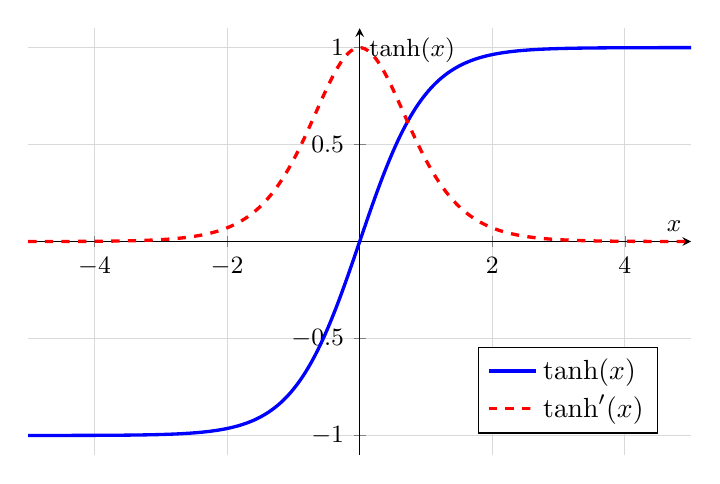
\begin{tikzpicture}
\begin{axis}[
    width=10cm,
    height=7cm,
    axis lines=middle,
    xlabel={$x$},
    ylabel={$\tanh(x)$},
    xmin=-5, xmax=5,
    ymin=-1.1, ymax=1.1,
    grid=major,
    grid style={gray!30},
    legend style={at={(0.95,0.05)},anchor=south east},
    legend cell align=left,
    smooth,
    samples=200,
    tick label style={font=\small},
    label style={font=\small},
]
\addplot[blue, very thick, domain=-5:5] {tanh(x)};
\addplot[red, dashed, very thick, domain=-5:5] {1-tanh(x)^2};
\legend{$\tanh(x)$, $\tanh'(x)$}
\end{axis}
\end{tikzpicture}
\end{center}

\textbf{3. ReLU 函数(Rectified Linear Unit)}

\textbf{数学公式}:
\begin{equation}
\text{ReLU}(x) = \max(0, x) = \begin{cases}
x & \text{if } x > 0 \\
0 & \text{if } x \leq 0
\end{cases}
\end{equation}

\textbf{导数}:
\begin{equation}
\text{ReLU}'(x) = \begin{cases}
1 & \text{if } x > 0 \\
0 & \text{if } x \leq 0
\end{cases}
\end{equation}

\textbf{输出范围}:$[0, +\infty)$

\textbf{函数图像}:

\begin{center}
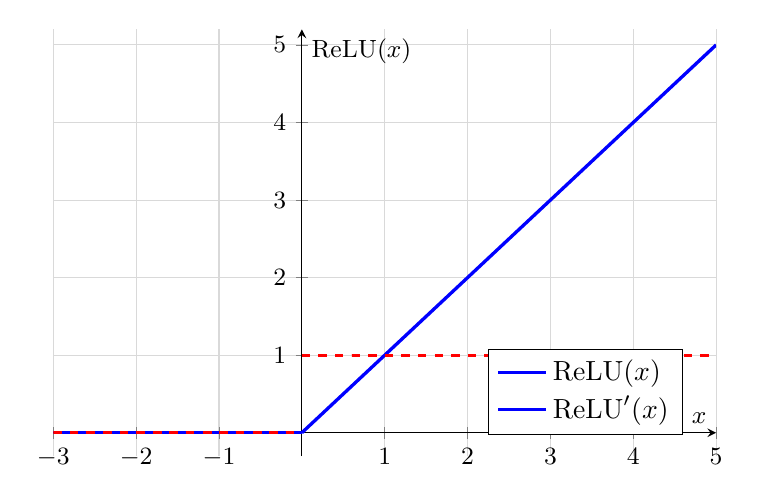
\begin{tikzpicture}
\begin{axis}[
    width=10cm,
    height=7cm,
    axis lines=middle,
    xlabel={$x$},
    ylabel={$\text{ReLU}(x)$},
    xmin=-3, xmax=5,
    ymin=-0.3, ymax=5.2,
    grid=major,
    grid style={gray!30},
    legend style={at={(0.95,0.05)},anchor=south east},
    legend cell align=left,
    samples=200,
    tick label style={font=\small},
    label style={font=\small},
]
\addplot[blue, very thick, domain=-3:0] {0};
\addplot[blue, very thick, domain=0:5] {x};
\addplot[red, dashed, very thick, domain=-3:0] {0};
\addplot[red, dashed, very thick, domain=0:5] {1};
\legend{$\text{ReLU}(x)$, $\text{ReLU}'(x)$}
\end{axis}
\end{tikzpicture}
\end{center}

\textbf{用处}:
\begin{itemize}
    \item 深度神经网络隐藏层的首选激活函数
    \item CNN、MLP 等大多数现代神经网络架构
    \item 需要稀疏激活的场景
\end{itemize}

\textbf{为什么用 ReLU}:
\begin{itemize}
    \item \textbf{缓解梯度消失}:在正区间梯度恒为1,不会衰减
    \item \textbf{计算高效}:只需比较和选择操作,计算速度快
    \item \textbf{稀疏激活}:约50\%的神经元会被激活,提高计算效率
    \item \textbf{生物学合理性}:模拟生物神经元的单侧抑制特性
\end{itemize}

\textbf{缺点}:
\begin{itemize}
    \item \textbf{死亡 ReLU 问题}:如果神经元输出始终为负,梯度为0,无法更新
    \item \textbf{非零中心}:输出均值不为0
    \item \textbf{无界}:输出可以无限大,可能导致数值不稳定
\end{itemize}

\textbf{4. Leaky ReLU}

\textbf{数学公式}:
\begin{equation}
\text{LeakyReLU}(x) = \max(\alpha x, x) = \begin{cases}
x & \text{if } x > 0 \\
\alpha x & \text{if } x \leq 0
\end{cases}
\end{equation}

其中 $\alpha$ 是小的正数(通常取 0.01)。

\textbf{导数}:
\begin{equation}
\text{LeakyReLU}'(x) = \begin{cases}
1 & \text{if } x > 0 \\
\alpha & \text{if } x \leq 0
\end{cases}
\end{equation}

\textbf{用处}:
\begin{itemize}
    \item 解决 ReLU 的死亡神经元问题
    \item 需要负值输出的场景
    \item 对梯度消失敏感的网络
\end{itemize}

\textbf{为什么用 Leaky ReLU}:
\begin{itemize}
    \item \textbf{避免死亡神经元}:负区间有小的梯度,神经元不会完全"死亡"
    \item \textbf{保持 ReLU 优点}:正区间仍保持线性,计算高效
    \item \textbf{更好的梯度流}:负区间也有梯度,信息可以反向传播
\end{itemize}

\textbf{函数图像}($\alpha = 0.01$):

\begin{center}
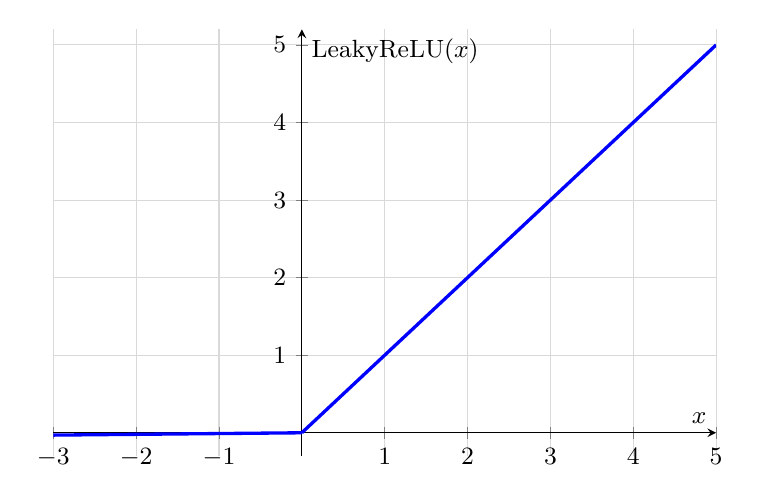
\begin{tikzpicture}
\begin{axis}[
    width=10cm,
    height=7cm,
    axis lines=middle,
    xlabel={$x$},
    ylabel={$\text{LeakyReLU}(x)$},
    xmin=-3, xmax=5,
    ymin=-0.3, ymax=5.2,
    grid=major,
    grid style={gray!30},
    smooth,
    samples=200,
    tick label style={font=\small},
    label style={font=\small},
]
\addplot[blue, very thick, domain=-3:0] {0.01*x};
\addplot[blue, very thick, domain=0:5] {x};
\end{axis}
\end{tikzpicture}
\end{center}

\textbf{5. ELU(Exponential Linear Unit)}

\textbf{数学公式}:
\begin{equation}
\text{ELU}(x) = \begin{cases}
x & \text{if } x > 0 \\
\alpha(e^x - 1) & \text{if } x \leq 0
\end{cases}
\end{equation}

其中 $\alpha$ 通常取 1.0。

\textbf{用处}:
\begin{itemize}
    \item 需要平滑负值输出的场景
    \item 对噪声敏感的任务
    \item 需要零均值输出的网络
\end{itemize}

\textbf{为什么用 ELU}:
\begin{itemize}
    \item \textbf{平滑性}:负区间平滑,避免 ReLU 的不连续性
    \item \textbf{零均值}:输出均值接近0,有助于训练
    \item \textbf{负值处理}:负区间有梯度,避免死亡神经元
\end{itemize}

\textbf{函数图像}($\alpha = 1.0$):

\begin{center}
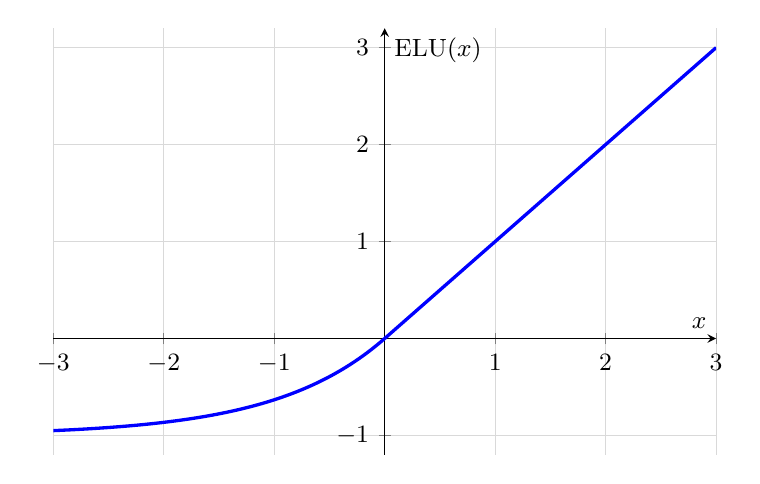
\begin{tikzpicture}
\begin{axis}[
    width=10cm,
    height=7cm,
    axis lines=middle,
    xlabel={$x$},
    ylabel={$\text{ELU}(x)$},
    xmin=-3, xmax=3,
    ymin=-1.2, ymax=3.2,
    grid=major,
    grid style={gray!30},
    smooth,
    samples=200,
    tick label style={font=\small},
    label style={font=\small},
]
\addplot[blue, very thick, domain=-3:0] {exp(x)-1};
\addplot[blue, very thick, domain=0:3] {x};
\end{axis}
\end{tikzpicture}
\end{center}

\textbf{6. Softmax 函数}

\textbf{数学公式}:
\begin{equation}
\text{softmax}(\mathbf{x})_i = \frac{e^{x_i}}{\sum_{j=1}^C e^{x_j}}
\end{equation}

其中 $C$ 是类别数,$\mathbf{x} \in \mathbb{R}^C$。

\textbf{输出范围}:$(0, 1)$,且 $\sum_{i=1}^C \text{softmax}(\mathbf{x})_i = 1$

\textbf{用处}:
\begin{itemize}
    \item 多分类任务的输出层
    \item 需要输出概率分布的场景
    \item 注意力机制中的注意力权重计算
\end{itemize}

\textbf{为什么用 Softmax}:
\begin{itemize}
    \item \textbf{概率分布}:输出是有效的概率分布,总和为1
    \item \textbf{与交叉熵配合}:与交叉熵损失函数配合使用,梯度形式简单
    \item \textbf{可解释性}:输出可以解释为各类别的概率
\end{itemize}

\subsubsection{激活函数选择指南}

\textbf{激活函数选择指南}:

\begin{itemize}
    \item \textbf{Sigmoid}:
    \begin{itemize}
        \item 适用场景:二分类输出层、门控机制
        \item 选择原因:输出概率、历史原因
    \end{itemize}
    
    \item \textbf{Tanh}:
    \begin{itemize}
        \item 适用场景:RNN 隐藏层、需要零中心化
        \item 选择原因:零均值、比 Sigmoid 更好
    \end{itemize}
    
    \item \textbf{ReLU}:
    \begin{itemize}
        \item 适用场景:深度网络隐藏层(首选)
        \item 选择原因:缓解梯度消失、计算高效
    \end{itemize}
    
    \item \textbf{Leaky ReLU}:
    \begin{itemize}
        \item 适用场景:解决死亡神经元问题
        \item 选择原因:负区间有梯度
    \end{itemize}
    
    \item \textbf{ELU}:
    \begin{itemize}
        \item 适用场景:需要平滑负值输出
        \item 选择原因:平滑、零均值
    \end{itemize}
    
    \item \textbf{Softmax}:
    \begin{itemize}
        \item 适用场景:多分类输出层
        \item 选择原因:概率分布、与交叉熵配合
    \end{itemize}
\end{itemize}

\textbf{应用场景}:
\begin{example}[手写数字识别]
MNIST 数据集是经典的图像分类任务,使用 MLP 可以达到较高的准确率。输入是 $28 \times 28 = 784$ 维的像素向量,输出是 10 个类别的概率分布。
\end{example}

\subsection{前向传播}

前向传播(Forward Propagation)是神经网络从输入到输出的计算过程。

\begin{algorithm}
\caption{前向传播算法}
\begin{algorithmic}[1]
\REQUIRE 输入 $\mathbf{x}$,网络参数 $\{\mathbf{W}^{(l)}, \mathbf{b}^{(l)}\}_{l=1}^L$
\ENSURE 输出 $\mathbf{y}$
\STATE $\mathbf{h}^{(0)} \leftarrow \mathbf{x}$
\FOR{$l = 1$ to $L-1$}
    \STATE $\mathbf{z}^{(l)} \leftarrow \mathbf{W}^{(l)} \mathbf{h}^{(l-1)} + \mathbf{b}^{(l)}$
    \STATE $\mathbf{h}^{(l)} \leftarrow \sigma(\mathbf{z}^{(l)})$
\ENDFOR
\STATE $\mathbf{z}^{(L)} \leftarrow \mathbf{W}^{(L)} \mathbf{h}^{(L-1)} + \mathbf{b}^{(L)}$
\STATE $\mathbf{y} \leftarrow \mathbf{z}^{(L)}$(或应用 softmax 等函数)
\end{algorithmic}
\end{algorithm}

\textbf{计算复杂度}:对于 $L$ 层网络,每层有 $n_l$ 个神经元,前向传播的时间复杂度为 $O(\sum_{l=1}^L n_{l-1} n_l)$。

\subsection{反向传播}

反向传播(Backpropagation)是训练神经网络的核心算法,通过链式法则计算损失函数对网络参数的梯度。

\begin{definition}[反向传播]
给定损失函数 $\mathcal{L}(\mathbf{y}, \hat{\mathbf{y}})$,反向传播算法计算梯度 $\frac{\partial \mathcal{L}}{\partial \mathbf{W}^{(l)}}$ 和 $\frac{\partial \mathcal{L}}{\partial \mathbf{b}^{(l)}}$。

对于输出层:
\begin{equation}
\frac{\partial \mathcal{L}}{\partial \mathbf{z}^{(L)}} = \frac{\partial \mathcal{L}}{\partial \mathbf{y}}
\end{equation}

对于隐藏层 $l = L-1, L-2, \ldots, 1$:
\begin{align}
\frac{\partial \mathcal{L}}{\partial \mathbf{h}^{(l)}} &= (\mathbf{W}^{(l+1)})^T \frac{\partial \mathcal{L}}{\partial \mathbf{z}^{(l+1)}} \\
\frac{\partial \mathcal{L}}{\partial \mathbf{z}^{(l)}} &= \frac{\partial \mathcal{L}}{\partial \mathbf{h}^{(l)}} \odot \sigma'(\mathbf{z}^{(l)}) \\
\frac{\partial \mathcal{L}}{\partial \mathbf{W}^{(l)}} &= \frac{\partial \mathcal{L}}{\partial \mathbf{z}^{(l)}} (\mathbf{h}^{(l-1)})^T \\
\frac{\partial \mathcal{L}}{\partial \mathbf{b}^{(l)}} &= \frac{\partial \mathcal{L}}{\partial \mathbf{z}^{(l)}}
\end{align}

其中,$\odot$ 表示逐元素相乘(Hadamard 积),$\sigma'$ 是激活函数的导数。
\end{definition}

\begin{algorithm}
\caption{反向传播算法}
\begin{algorithmic}[1]
\REQUIRE 前向传播的输出 $\mathbf{y}$,真实标签 $\hat{\mathbf{y}}$,损失函数 $\mathcal{L}$
\ENSURE 梯度 $\{\frac{\partial \mathcal{L}}{\partial \mathbf{W}^{(l)}}, \frac{\partial \mathcal{L}}{\partial \mathbf{b}^{(l)}}\}_{l=1}^L$
\STATE 计算输出层梯度:$\delta^{(L)} = \frac{\partial \mathcal{L}}{\partial \mathbf{z}^{(L)}}$
\FOR{$l = L-1$ down to $1$}
    \STATE $\delta^{(l)} = (\mathbf{W}^{(l+1)})^T \delta^{(l+1)} \odot \sigma'(\mathbf{z}^{(l)})$
    \STATE $\frac{\partial \mathcal{L}}{\partial \mathbf{W}^{(l)}} = \delta^{(l)} (\mathbf{h}^{(l-1)})^T$
    \STATE $\frac{\partial \mathcal{L}}{\partial \mathbf{b}^{(l)}} = \delta^{(l)}$
\ENDFOR
\end{algorithmic}
\end{algorithm}

\textbf{梯度消失问题}:在深层网络中,梯度在反向传播过程中可能指数级衰减,导致底层参数难以更新。使用 ReLU 激活函数、残差连接、批量归一化等技术可以缓解这一问题。

\subsection{损失函数}

损失函数(Loss Function)用于衡量模型预测值与真实值之间的差异,是训练神经网络的核心目标函数。选择合适的损失函数对模型性能至关重要。

\subsubsection{回归任务的损失函数}

\textbf{均方误差(Mean Squared Error, MSE)}:
\begin{equation}
\mathcal{L}_{MSE} = \frac{1}{n} \sum_{i=1}^n (y_i - \hat{y}_i)^2
\end{equation}

其中,$y_i$ 是真实值,$\hat{y}_i$ 是预测值,$n$ 是样本数量。

\textbf{特点}:
\begin{itemize}
    \item 对大误差敏感,惩罚较大
    \item 梯度与误差成正比,训练稳定
    \item 适用于回归问题,假设误差服从高斯分布
\end{itemize}

\textbf{函数图像}(假设真实值 $y=0$):

\begin{center}
\begin{tikzpicture}
\begin{axis}[
    width=10cm,
    height=7cm,
    axis lines=middle,
    xlabel={预测值 $\hat{y}$},
    ylabel={损失 $\mathcal{L}_{MSE}$},
    xmin=-3, xmax=3,
    ymin=0, ymax=10,
    grid=major,
    grid style={gray!30},
    smooth,
    samples=200,
    tick label style={font=\small},
    label style={font=\small},
]
\addplot[blue, very thick, domain=-3:3] {x^2};
\end{axis}
\end{tikzpicture}
\end{center}

\textbf{平均绝对误差(Mean Absolute Error, MAE)}:
\begin{equation}
\mathcal{L}_{MAE} = \frac{1}{n} \sum_{i=1}^n |y_i - \hat{y}_i|
\end{equation}

\textbf{特点}:
\begin{itemize}
    \item 对大误差不敏感,对异常值更鲁棒
    \item 梯度为常数($\pm 1$),训练可能不稳定
    \item 适用于需要鲁棒性的回归问题
\end{itemize}

\textbf{函数图像}(假设真实值 $y=0$):

\begin{center}
\begin{tikzpicture}
\begin{axis}[
    width=10cm,
    height=7cm,
    axis lines=middle,
    xlabel={预测值 $\hat{y}$},
    ylabel={损失 $\mathcal{L}_{MAE}$},
    xmin=-3, xmax=3,
    ymin=0, ymax=3.5,
    grid=major,
    grid style={gray!30},
    samples=200,
    tick label style={font=\small},
    label style={font=\small},
]
\addplot[blue, very thick, domain=-3:3] {abs(x)};
\end{axis}
\end{tikzpicture}
\end{center}

\textbf{Huber Loss}:结合 MSE 和 MAE 的优点:
\begin{equation}
\mathcal{L}_{Huber}(y, \hat{y}) = \begin{cases}
\frac{1}{2}(y - \hat{y})^2 & \text{if } |y - \hat{y}| \leq \delta \\
\delta |y - \hat{y}| - \frac{1}{2}\delta^2 & \text{otherwise}
\end{cases}
\end{equation}

其中,$\delta$ 是超参数(通常取 1.0)。当误差小于 $\delta$ 时,使用 MSE;否则使用 MAE。

\textbf{函数图像}(假设真实值 $y=0$,$\delta=1.0$):

\begin{center}
\begin{tikzpicture}
\begin{axis}[
    width=10cm,
    height=7cm,
    axis lines=middle,
    xlabel={预测值 $\hat{y}$},
    ylabel={损失 $\mathcal{L}_{Huber}$},
    xmin=-3, xmax=3,
    ymin=0, ymax=3.5,
    grid=major,
    grid style={gray!30},
    samples=200,
    tick label style={font=\small},
    label style={font=\small},
]
\addplot[blue, very thick, domain=-1:1] {0.5*x^2};
\addplot[blue, very thick, domain=-3:-1] {abs(x)-0.5};
\addplot[blue, very thick, domain=1:3] {abs(x)-0.5};
\end{axis}
\end{tikzpicture}
\end{center}

\subsubsection{分类任务的损失函数}

\textbf{交叉熵损失(Cross-Entropy Loss)}:
对于二分类问题:
\begin{equation}
\mathcal{L}_{CE} = -\frac{1}{n} \sum_{i=1}^n [y_i \log(\hat{y}_i) + (1-y_i) \log(1-\hat{y}_i)]
\end{equation}

对于多分类问题($C$ 个类别):
\begin{equation}
\mathcal{L}_{CE} = -\frac{1}{n} \sum_{i=1}^n \sum_{c=1}^C y_{i,c} \log(\hat{y}_{i,c})
\end{equation}

其中,$y_{i,c}$ 是真实标签的 one-hot 编码,$\hat{y}_{i,c}$ 是模型预测的概率。

\textbf{特点}:
\begin{itemize}
    \item 与 softmax 激活函数配合使用效果最佳
    \item 梯度形式简单:$\frac{\partial \mathcal{L}_{CE}}{\partial \hat{y}_i} = -\frac{y_i}{\hat{y}_i}$
    \item 适用于分类问题,假设输出服从多项分布
\end{itemize}

\textbf{函数图像}(二分类,真实标签 $y=1$):

\begin{center}
\begin{tikzpicture}
\begin{axis}[
    width=10cm,
    height=7cm,
    axis lines=middle,
    xlabel={预测概率 $\hat{y}$},
    ylabel={损失 $\mathcal{L}_{CE}$},
    xmin=0, xmax=1,
    ymin=0, ymax=5,
    grid=major,
    grid style={gray!30},
    smooth,
    samples=200,
    tick label style={font=\small},
    label style={font=\small},
]
\addplot[blue, very thick, domain=0.01:0.99] {-ln(x)};
\end{axis}
\end{tikzpicture}
\end{center}

\textbf{Focal Loss}:解决类别不平衡问题:
\begin{equation}
\mathcal{L}_{Focal} = -\alpha_t (1-p_t)^\gamma \log(p_t)
\end{equation}

其中,$p_t$ 是模型预测的正确类别的概率,$\alpha_t$ 是平衡因子,$\gamma$ 是聚焦参数(通常 $\gamma = 2$)。

\textbf{特点}:
\begin{itemize}
    \item $(1-p_t)^\gamma$ 项降低易分类样本的权重
    \item 专注于难分类样本,提高模型性能
    \item 在目标检测任务中广泛应用(如 RetinaNet)
\end{itemize}

\subsubsection{其他损失函数}

\textbf{对比损失(Contrastive Loss)}:用于学习相似性:
\begin{equation}
\mathcal{L}_{Contrastive} = \begin{cases}
\frac{1}{2} d^2 & \text{if } y = 1 \text{ (相似)} \\
\frac{1}{2} \max(0, m - d)^2 & \text{if } y = 0 \text{ (不相似)}
\end{cases}
\end{equation}

其中,$d$ 是两个样本的欧氏距离,$m$ 是边界参数(margin)。

\textbf{三元组损失(Triplet Loss)}:用于度量学习:
\begin{equation}
\mathcal{L}_{Triplet} = \max(0, d(a, p) - d(a, n) + m)
\end{equation}

其中,$a$ 是锚样本(anchor),$p$ 是正样本(positive),$n$ 是负样本(negative),$d(\cdot, \cdot)$ 是距离函数,$m$ 是边界。

\textbf{应用场景}:
\begin{itemize}
    \item 人脸识别:FaceNet 使用三元组损失
    \item 图像检索:学习图像的相似性表示
    \item 推荐系统:学习用户和物品的嵌入
\end{itemize}

\textbf{感知损失(Perceptual Loss)}:用于图像生成任务:
\begin{equation}
\mathcal{L}_{Perceptual} = \sum_{l} \lambda_l \|\phi_l(\hat{I}) - \phi_l(I)\|_2^2
\end{equation}

其中,$\phi_l$ 是预训练网络(如 VGG)的第 $l$ 层特征,$\lambda_l$ 是权重。

\textbf{应用场景}:
\begin{itemize}
    \item 图像超分辨率:SRGAN
    \item 风格迁移:保持内容的同时改变风格
    \item 图像修复:生成缺失区域
\end{itemize}

\subsubsection{损失函数的选择原则}

\begin{enumerate}
    \item \textbf{任务类型}:
    \begin{itemize}
        \item 回归任务:MSE、MAE、Huber Loss
        \item 二分类:二元交叉熵
        \item 多分类:多元交叉熵
        \item 多标签分类:二元交叉熵(每个类别独立)
    \end{itemize}
    
    \item \textbf{数据分布}:
    \begin{itemize}
        \item 类别不平衡:Focal Loss、加权交叉熵
        \item 异常值多:MAE、Huber Loss
        \item 高斯噪声:MSE
    \end{itemize}
    
    \item \textbf{训练稳定性}:
    \begin{itemize}
        \item 梯度爆炸风险:使用梯度裁剪
        \item 梯度消失:选择合适的激活函数和损失函数组合
    \end{itemize}
    
    \item \textbf{应用需求}:
    \begin{itemize}
        \item 需要可解释性:使用简单的损失函数
        \item 需要特定属性:使用定制损失函数(如感知损失)
    \end{itemize}
\end{enumerate}

\begin{remark}
在实际应用中,可以组合多个损失函数:
\begin{equation}
\mathcal{L}_{Total} = \lambda_1 \mathcal{L}_1 + \lambda_2 \mathcal{L}_2 + \cdots + \lambda_k \mathcal{L}_k
\end{equation}

其中,$\lambda_i$ 是各损失函数的权重,需要根据任务需求调整。
\end{remark}

\subsubsection{损失函数使用原因总结}

\textbf{常见损失函数的使用原因}:

\begin{itemize}
    \item \textbf{MSE(均方误差)}:
    \begin{itemize}
        \item 主要用途:回归任务
        \item 为什么用它:假设误差服从高斯分布,对大误差敏感,梯度稳定
    \end{itemize}
    
    \item \textbf{MAE(平均绝对误差)}:
    \begin{itemize}
        \item 主要用途:回归任务(异常值多)
        \item 为什么用它:对异常值鲁棒,梯度为常数
    \end{itemize}
    
    \item \textbf{Huber Loss}:
    \begin{itemize}
        \item 主要用途:回归任务(平衡鲁棒性和稳定性)
        \item 为什么用它:结合 MSE 和 MAE 优点,小误差用 MSE,大误差用 MAE
    \end{itemize}
    
    \item \textbf{交叉熵(Cross-Entropy)}:
    \begin{itemize}
        \item 主要用途:分类任务
        \item 为什么用它:与 softmax 配合,梯度形式简单,假设输出为多项分布
    \end{itemize}
    
    \item \textbf{Focal Loss}:
    \begin{itemize}
        \item 主要用途:类别不平衡的分类任务
        \item 为什么用它:降低易分类样本权重,专注于难样本
    \end{itemize}
    
    \item \textbf{对比损失(Contrastive Loss)}:
    \begin{itemize}
        \item 主要用途:相似性学习
        \item 为什么用它:学习样本间的相似性关系
    \end{itemize}
    
    \item \textbf{三元组损失(Triplet Loss)}:
    \begin{itemize}
        \item 主要用途:度量学习
        \item 为什么用它:学习样本间的相对距离关系
    \end{itemize}
    
    \item \textbf{感知损失(Perceptual Loss)}:
    \begin{itemize}
        \item 主要用途:图像生成
        \item 为什么用它:在特征空间计算损失,更符合人类感知
    \end{itemize}
\end{itemize}

\subsection{评估函数(评估指标)}

评估函数(Evaluation Metrics)用于衡量模型在测试集上的性能,与损失函数不同,评估函数通常更关注实际应用中的性能表现。

\subsubsection{分类任务的评估指标}

\textbf{1. 准确率(Accuracy)}

\textbf{数学公式}:
\begin{equation}
\text{Accuracy} = \frac{\text{正确预测数}}{\text{总样本数}} = \frac{TP + TN}{TP + TN + FP + FN}
\end{equation}

其中,TP(True Positive)是真阳性,TN(True Negative)是真阴性,FP(False Positive)是假阳性,FN(False Negative)是假阴性。

\textbf{用处}:
\begin{itemize}
    \item 类别平衡的分类任务
    \item 需要整体性能评估的场景
    \item 快速了解模型整体表现
\end{itemize}

\textbf{为什么用准确率}:
\begin{itemize}
    \item \textbf{直观易懂}:最直观的性能指标,容易理解
    \item \textbf{计算简单}:计算成本低,适合大规模评估
    \item \textbf{通用性强}:适用于所有分类任务
\end{itemize}

\textbf{缺点}:
\begin{itemize}
    \item \textbf{类别不平衡时失效}:如果99\%的样本是正类,预测全为正类也能达到99\%准确率
    \item \textbf{忽略错误类型}:不区分假阳性 and 假阴性
\end{itemize}

\textbf{2. 精确率(Precision)}

\textbf{数学公式}:
\begin{equation}
\text{Precision} = \frac{TP}{TP + FP}
\end{equation}

\textbf{用处}:
\begin{itemize}
    \item 需要减少假阳性的场景(如垃圾邮件检测)
    \item 关注"预测为正类的样本中,有多少是真的正类"
\end{itemize}

\textbf{为什么用精确率}:
\begin{itemize}
    \item \textbf{减少误报}:当假阳性代价高时,精确率更重要
    \item \textbf{资源有限}:当处理正类样本需要消耗资源时,精确率很重要
\end{itemize}

\textbf{3. 召回率(Recall)}

\textbf{数学公式}:
\begin{equation}
\text{Recall} = \frac{TP}{TP + FN} = \text{Sensitivity}
\end{equation}

\textbf{用处}:
\begin{itemize}
    \item 需要减少假阴性的场景(如疾病诊断)
    \item 关注"所有正类样本中,有多少被正确识别"
\end{itemize}

\textbf{为什么用召回率}:
\begin{itemize}
    \item \textbf{减少漏报}:当假阴性代价高时,召回率更重要
    \item \textbf{全面覆盖}:需要尽可能找到所有正类样本
\end{itemize}

\textbf{4. F1 分数(F1-Score)}

\textbf{数学公式}:
\begin{equation}
F_1 = \frac{2 \times \text{Precision} \times \text{Recall}}{\text{Precision} + \text{Recall}} = \frac{2TP}{2TP + FP + FN}
\end{equation}

\textbf{用处}:
\begin{itemize}
    \item 需要平衡精确率和召回率的场景
    \item 类别不平衡的分类任务
    \item 单一指标评估模型性能
\end{itemize}

\textbf{为什么用 F1 分数}:
\begin{itemize}
    \item \textbf{平衡指标}:综合考虑精确率和召回率
    \item \textbf{调和平均数}:使用调和平均数,对低值更敏感
    \item \textbf{单一指标}:用一个数字概括模型性能,便于比较
\end{itemize}

\textbf{5. ROC 曲线和 AUC}

\textbf{ROC 曲线}:以假阳性率(FPR)为横轴,真阳性率(TPR,即召回率)为纵轴的曲线。

\textbf{AUC(Area Under Curve)}:ROC 曲线下的面积。

\textbf{数学公式}:
\begin{align}
\text{FPR} &= \frac{FP}{FP + TN} \\
\text{TPR} &= \frac{TP}{TP + FN} = \text{Recall}
\end{align}

\textbf{用处}:
\begin{itemize}
    \item 二分类任务的性能评估
    \item 需要比较不同模型的整体性能
    \item 类别不平衡的任务
\end{itemize}

\textbf{为什么用 AUC}:
\begin{itemize}
    \item \textbf{阈值无关}:不依赖于分类阈值,评估模型整体性能
    \item \textbf{类别不平衡鲁棒}:对类别不平衡相对鲁棒
    \item \textbf{概率解释}:AUC 可以解释为"随机选择一个正样本和一个负样本,模型对正样本的预测概率大于负样本的概率"
\end{itemize}

\subsubsection{回归任务的评估指标}

\textbf{1. 均方误差(MSE)}

\textbf{数学公式}:
\begin{equation}
\text{MSE} = \frac{1}{n} \sum_{i=1}^n (y_i - \hat{y}_i)^2
\end{equation}

\textbf{用处}:
\begin{itemize}
    \item 回归任务的标准评估指标
    \item 需要惩罚大误差的场景
\end{itemize}

\textbf{为什么用 MSE}:
\begin{itemize}
    \item \textbf{标准指标}:最常用的回归评估指标
    \item \textbf{可导性}:可导,便于优化
    \item \textbf{大误差敏感}:对大误差敏感,符合实际需求
\end{itemize}

\textbf{2. 均方根误差(RMSE)}

\textbf{数学公式}:
\begin{equation}
\text{RMSE} = \sqrt{\text{MSE}} = \sqrt{\frac{1}{n} \sum_{i=1}^n (y_i - \hat{y}_i)^2}
\end{equation}

\textbf{用处}:
\begin{itemize}
    \item 需要与原数据相同量纲的评估指标
    \item 更直观的误差表示
\end{itemize}

\textbf{为什么用 RMSE}:
\begin{itemize}
    \item \textbf{量纲一致}:与原数据量纲相同,更直观
    \item \textbf{可解释性}:可以直接理解为"平均误差"
\end{itemize}

\textbf{3. 平均绝对误差(MAE)}

\textbf{数学公式}:
\begin{equation}
\text{MAE} = \frac{1}{n} \sum_{i=1}^n |y_i - \hat{y}_i|
\end{equation}

\textbf{用处}:
\begin{itemize}
    \item 需要鲁棒性评估的场景
    \item 异常值较多的数据
\end{itemize}

\textbf{为什么用 MAE}:
\begin{itemize}
    \item \textbf{鲁棒性}:对异常值不敏感
    \item \textbf{直观性}:直接表示平均误差,易于理解
\end{itemize}

\textbf{4. 决定系数(R² Score)}

\textbf{数学公式}:
\begin{equation}
R^2 = 1 - \frac{\sum_{i=1}^n (y_i - \hat{y}_i)^2}{\sum_{i=1}^n (y_i - \bar{y})^2} = 1 - \frac{\text{SS}_{res}}{\text{SS}_{tot}}
\end{equation}

其中 $\bar{y} = \frac{1}{n}\sum_{i=1}^n y_i$ 是真实值的均值。

\textbf{输出范围}:$(-\infty, 1]$,越接近1越好。

\textbf{用处}:
\begin{itemize}
    \item 需要相对性能评估的场景
    \item 比较不同模型的解释能力
\end{itemize}

\textbf{为什么用 R²}:
\begin{itemize}
    \item \textbf{相对性能}:表示模型相对于简单均值预测的改进程度
    \item \textbf{标准化}:值域固定,便于比较不同数据集上的模型
    \item \textbf{可解释性}:可以解释为"模型解释了多少方差"
\end{itemize}

\subsubsection{评估指标选择指南}

\textbf{评估指标选择指南}:

\begin{itemize}
    \item \textbf{准确率(Accuracy)}:
    \begin{itemize}
        \item 适用任务:类别平衡的分类任务
        \item 选择原因:直观易懂,计算简单
    \end{itemize}
    
    \item \textbf{精确率(Precision)}:
    \begin{itemize}
        \item 适用任务:需要减少假阳性
        \item 选择原因:关注预测正类的准确性
    \end{itemize}
    
    \item \textbf{召回率(Recall)}:
    \begin{itemize}
        \item 适用任务:需要减少假阴性
        \item 选择原因:关注找到所有正类
    \end{itemize}
    
    \item \textbf{F1 分数}:
    \begin{itemize}
        \item 适用任务:需要平衡精确率和召回率
        \item 选择原因:单一指标,平衡两者
    \end{itemize}
    
    \item \textbf{AUC(ROC 曲线下面积)}:
    \begin{itemize}
        \item 适用任务:二分类任务,类别不平衡
        \item 选择原因:阈值无关,整体性能
    \end{itemize}
    
    \item \textbf{MSE/RMSE(均方误差/均方根误差)}:
    \begin{itemize}
        \item 适用任务:回归任务
        \item 选择原因:标准指标,大误差敏感
    \end{itemize}
    
    \item \textbf{MAE(平均绝对误差)}:
    \begin{itemize}
        \item 适用任务:回归任务(异常值多)
        \item 选择原因:鲁棒性强
    \end{itemize}
    
    \item \textbf{R²(决定系数)}:
    \begin{itemize}
        \item 适用任务:回归任务(相对性能)
        \item 选择原因:标准化,可解释性强
    \end{itemize}
\end{itemize}

\section{简易神经网络完整示例}

本节通过一个完整的简易神经网络示例,展示深度学习的核心概念,包括编码(Encode)、解码(Decode)、训练和推理的全过程。

\subsection{网络架构设计}

\textbf{任务}:使用一个简单的三层神经网络进行二分类任务(如判断邮件是否为垃圾邮件)。

\textbf{网络结构}:
\begin{itemize}
    \item \textbf{输入层}:$d_{in} = 4$ 个特征(如邮件的关键词频率)
    \item \textbf{隐藏层1}:$h_1 = 8$ 个神经元,使用 ReLU 激活函数
    \item \textbf{隐藏层2}:$h_2 = 4$ 个神经元,使用 ReLU 激活函数
    \item \textbf{输出层}:$d_{out} = 1$ 个神经元,使用 Sigmoid 激活函数(输出概率)
\end{itemize}

\textbf{数学表示}:

对于输入 $\mathbf{x} \in \mathbb{R}^4$,网络的前向传播为:
\begin{align}
\mathbf{h}^{(1)} &= \text{ReLU}(\mathbf{W}^{(1)}\mathbf{x} + \mathbf{b}^{(1)}) \quad \mathbf{W}^{(1)} \in \mathbb{R}^{8 \times 4}, \mathbf{b}^{(1)} \in \mathbb{R}^8 \\
\mathbf{h}^{(2)} &= \text{ReLU}(\mathbf{W}^{(2)}\mathbf{h}^{(1)} + \mathbf{b}^{(2)}) \quad \mathbf{W}^{(2)} \in \mathbb{R}^{4 \times 8}, \mathbf{b}^{(2)} \in \mathbb{R}^4 \\
\hat{y} &= \sigma(\mathbf{W}^{(3)}\mathbf{h}^{(2)} + \mathbf{b}^{(3)}) \quad \mathbf{W}^{(3)} \in \mathbb{R}^{1 \times 4}, \mathbf{b}^{(3)} \in \mathbb{R}^1
\end{align}

其中 $\sigma$ 是 Sigmoid 函数:$\sigma(x) = \frac{1}{1 + e^{-x}}$。

\subsection{从零实现神经网络}

\textbf{完整代码实现}:

\begin{lstlisting}[caption=简易神经网络完整实现(使用 NumPy)]
import numpy as np
import pandas as pd

class SimpleNeuralNetwork:
    """简易三层神经网络"""
    
    def __init__(self, input_size=4, hidden1_size=8, hidden2_size=4, output_size=1):
        """
        初始化神经网络
        
        参数:
            input_size: 输入特征维度
            hidden1_size: 第一个隐藏层神经元数量
            hidden2_size: 第二个隐藏层神经元数量
            output_size: 输出维度
        """
        # 初始化权重矩阵(使用 Xavier 初始化)
        self.W1 = np.random.randn(hidden1_size, input_size) * np.sqrt(2.0 / input_size)
        self.b1 = np.zeros((hidden1_size, 1))
        
        self.W2 = np.random.randn(hidden2_size, hidden1_size) * np.sqrt(2.0 / hidden1_size)
        self.b2 = np.zeros((hidden2_size, 1))
        
        self.W3 = np.random.randn(output_size, hidden2_size) * np.sqrt(2.0 / hidden2_size)
        self.b3 = np.zeros((output_size, 1))
    
    def relu(self, x):
        """ReLU 激活函数"""
        return np.maximum(0, x)
    
    def relu_derivative(self, x):
        """ReLU 的导数"""
        return (x > 0).astype(float)
    
    def sigmoid(self, x):
        """Sigmoid 激活函数"""
        # 防止溢出
        x = np.clip(x, -500, 500)
        return 1 / (1 + np.exp(-x))
    
    def sigmoid_derivative(self, x):
        """Sigmoid 的导数"""
        s = self.sigmoid(x)
        return s * (1 - s)
    
    def forward(self, X):
        """
        前向传播(Encode)
        
        参数:
            X: 输入数据 (batch_size, input_size)
        
        返回:
            y_pred: 预测输出 (batch_size, output_size)
            cache: 中间结果(用于反向传播)
        """
        # 输入层 → 隐藏层1
        self.z1 = X.dot(self.W1.T) + self.b1.T  # (batch_size, hidden1_size)
        self.a1 = self.relu(self.z1)  # 激活
        
        # 隐藏层1 → 隐藏层2
        self.z2 = self.a1.dot(self.W2.T) + self.b2.T  # (batch_size, hidden2_size)
        self.a2 = self.relu(self.z2)  # 激活
        
        # 隐藏层2 → 输出层
        self.z3 = self.a2.dot(self.W3.T) + self.b3.T  # (batch_size, output_size)
        self.a3 = self.sigmoid(self.z3)  # 激活(输出概率)
        
        return self.a3
    
    def backward(self, X, y, y_pred):
        """
        反向传播(计算梯度)
        
        参数:
            X: 输入数据 (batch_size, input_size)
            y: 真实标签 (batch_size, 1)
            y_pred: 预测输出 (batch_size, output_size)
        """
        m = X.shape[0]  # 批次大小
        
        # 输出层误差
        dz3 = y_pred - y  # (batch_size, output_size)
        dW3 = (1/m) * dz3.T.dot(self.a2)  # (output_size, hidden2_size)
        db3 = (1/m) * np.sum(dz3, axis=0, keepdims=True).T  # (output_size, 1)
        
        # 隐藏层2误差
        da2 = dz3.dot(self.W3)  # (batch_size, hidden2_size)
        dz2 = da2 * self.relu_derivative(self.z2)  # 链式法则
        dW2 = (1/m) * dz2.T.dot(self.a1)  # (hidden2_size, hidden1_size)
        db2 = (1/m) * np.sum(dz2, axis=0, keepdims=True).T  # (hidden2_size, 1)
        
        # 隐藏层1误差
        da1 = dz2.dot(self.W2)  # (batch_size, hidden1_size)
        dz1 = da1 * self.relu_derivative(self.z1)  # 链式法则
        dW1 = (1/m) * dz1.T.dot(X)  # (hidden1_size, input_size)
        db1 = (1/m) * np.sum(dz1, axis=0, keepdims=True).T  # (hidden1_size, 1)
        
        return dW1, db1, dW2, db2, dW3, db3
    
    def update_parameters(self, dW1, db1, dW2, db2, dW3, db3, learning_rate):
        """更新参数(梯度下降)"""
        self.W1 -= learning_rate * dW1
        self.b1 -= learning_rate * db1
        self.W2 -= learning_rate * dW2
        self.b2 -= learning_rate * db2
        self.W3 -= learning_rate * dW3
        self.b3 -= learning_rate * db3
    
    def compute_loss(self, y_pred, y):
        """
        计算损失函数(二元交叉熵)
        
        数学公式:
        L = -\frac{1}{m}\sum_{i=1}^m [y_i \log(\hat{y}_i) + (1-y_i)\log(1-\hat{y}_i)]
        """
        m = y.shape[0]
        # 防止 log(0)
        epsilon = 1e-15
        y_pred = np.clip(y_pred, epsilon, 1 - epsilon)
        loss = -(1/m) * np.sum(y * np.log(y_pred) + (1 - y) * np.log(1 - y_pred))
        return loss
    
    def train(self, X_train, y_train, epochs=1000, learning_rate=0.01, verbose=True):
        """
        训练神经网络
        
        参数:
            X_train: 训练数据 (n_samples, input_size)
            y_train: 训练标签 (n_samples, 1)
            epochs: 训练轮数
            learning_rate: 学习率
            verbose: 是否打印训练过程
        """
        losses = []
        
        for epoch in range(epochs):
            # 前向传播
            y_pred = self.forward(X_train)
            
            # 计算损失
            loss = self.compute_loss(y_pred, y_train)
            losses.append(loss)
            
            # 反向传播
            dW1, db1, dW2, db2, dW3, db3 = self.backward(X_train, y_train, y_pred)
            
            # 更新参数
            self.update_parameters(dW1, db1, dW2, db2, dW3, db3, learning_rate)
            
            # 打印训练进度
            if verbose and (epoch + 1) % 100 == 0:
                print(f"Epoch {epoch+1}/{epochs}, Loss: {loss:.4f}")
        
        return losses
    
    def predict(self, X):
        """
        预测(Decode/推理)
        
        参数:
            X: 输入数据 (n_samples, input_size)
        
        返回:
            predictions: 预测结果 (n_samples, 1),值在 [0, 1] 之间
        """
        y_pred = self.forward(X)
        return y_pred
    
    def predict_class(self, X, threshold=0.5):
        """
        预测类别(二分类)
        
        参数:
            X: 输入数据
            threshold: 分类阈值
        
        返回:
            classes: 预测类别 (0 或 1)
        """
        y_pred = self.predict(X)
        return (y_pred > threshold).astype(int)

# 使用示例
# 1. 准备数据(编码:将原始数据转换为数值特征)
np.random.seed(42)
n_samples = 1000
X_train = np.random.randn(n_samples, 4)  # 4个特征
y_train = (X_train.sum(axis=1) > 0).astype(float).reshape(-1, 1)  # 简单二分类任务

# 2. 创建和训练模型
model = SimpleNeuralNetwork(input_size=4, hidden1_size=8, hidden2_size=4, output_size=1)
losses = model.train(X_train, y_train, epochs=1000, learning_rate=0.01)

# 3. 预测(解码:将网络输出转换为类别)
X_test = np.random.randn(10, 4)
predictions = model.predict(X_test)
classes = model.predict_class(X_test)

print("\n预测结果:")
print(f"预测概率: {predictions.flatten()}")
print(f"预测类别: {classes.flatten()}")
\end{lstlisting}

\subsection{概念对应关系}

通过这个简易神经网络示例,我们可以清楚地看到深度学习各个概念的对应关系:

\textbf{深度学习概念在代码中的对应}:

\begin{itemize}
    \item \textbf{输入层}:\texttt{X}(输入数据矩阵)
    \item \textbf{隐藏层1}:\texttt{self.a1}(8个神经元)
    \item \textbf{隐藏层2}:\texttt{self.a2}(4个神经元)
    \item \textbf{输出层}:\texttt{self.a3}(1个神经元,输出概率)
    \item \textbf{权重矩阵}:\texttt{self.W1, self.W2, self.W3}
    \item \textbf{偏置向量}:\texttt{self.b1, self.b2, self.b3}
    \item \textbf{激活函数}:\texttt{relu(), sigmoid()}
    \item \textbf{前向传播(Encode)}:\texttt{forward()} 方法
    \item \textbf{反向传播}:\texttt{backward()} 方法
    \item \textbf{损失函数}:\texttt{compute\_loss()}(交叉熵)
    \item \textbf{梯度下降}:\texttt{update\_parameters()}
    \item \textbf{训练}:\texttt{train()} 方法
    \item \textbf{推理(Decode)}:\texttt{predict()} 和 \texttt{predict\_class()}
\end{itemize}

\subsection{网络结构图示}

\textbf{网络架构图}:

\begin{center}
\textbf{输入层 (4个神经元)} $\rightarrow$ \textbf{隐藏层1 (8个神经元, ReLU)} $\rightarrow$ \textbf{隐藏层2 (4个神经元, ReLU)} $\rightarrow$ \textbf{输出层 (1个神经元, Sigmoid)}
\end{center}

\textbf{详细结构图示}:

\begin{center}
\vspace{0.5cm}
\begin{tikzpicture}[scale=1.0]
% 定义神经元间距(增大间距避免重叠)
\def\spacing{1.5}

% 输入层 - 4个神经元,关于横轴对称
% 位置:-2.25, -0.75, 0.75, 2.25
\node[circle, draw, minimum size=0.8cm, fill=blue!20] (x1) at (0, -2.25) {$x_1$};
\node[circle, draw, minimum size=0.8cm, fill=blue!20] (x2) at (0, -0.75) {$x_2$};
\node[circle, draw, minimum size=0.8cm, fill=blue!20] (x3) at (0, 0.75) {$x_3$};
\node[circle, draw, minimum size=0.8cm, fill=blue!20] (x4) at (0, 2.25) {$x_4$};

% 隐藏层1 - 8个神经元,关于横轴对称
% 位置:-5.25, -3.75, -2.25, -0.75, 0.75, 2.25, 3.75, 5.25
\node[circle, draw, minimum size=0.7cm, fill=green!20] (h11) at (4, -5.25) {$h_1^{(1)}$};
\node[circle, draw, minimum size=0.7cm, fill=green!20] (h12) at (4, -3.75) {$h_1^{(2)}$};
\node[circle, draw, minimum size=0.7cm, fill=green!20] (h13) at (4, -2.25) {$h_1^{(3)}$};
\node[circle, draw, minimum size=0.7cm, fill=green!20] (h14) at (4, -0.75) {$h_1^{(4)}$};
\node[circle, draw, minimum size=0.7cm, fill=green!20] (h15) at (4, 0.75) {$h_1^{(5)}$};
\node[circle, draw, minimum size=0.7cm, fill=green!20] (h16) at (4, 2.25) {$h_1^{(6)}$};
\node[circle, draw, minimum size=0.7cm, fill=green!20] (h17) at (4, 3.75) {$h_1^{(7)}$};
\node[circle, draw, minimum size=0.7cm, fill=green!20] (h18) at (4, 5.25) {$h_1^{(8)}$};

% 隐藏层2 - 4个神经元,关于横轴对称
% 位置:-2.25, -0.75, 0.75, 2.25
\node[circle, draw, minimum size=0.7cm, fill=orange!20] (h21) at (8, -2.25) {$h_2^{(1)}$};
\node[circle, draw, minimum size=0.7cm, fill=orange!20] (h22) at (8, -0.75) {$h_2^{(2)}$};
\node[circle, draw, minimum size=0.7cm, fill=orange!20] (h23) at (8, 0.75) {$h_2^{(3)}$};
\node[circle, draw, minimum size=0.7cm, fill=orange!20] (h24) at (8, 2.25) {$h_2^{(4)}$};

% 输出层 - 1个神经元,在横轴上
\node[circle, draw, minimum size=0.8cm, fill=red!20] (y) at (12, 0) {$\hat{y}$};

% 输入层到隐藏层1的连接
\foreach \i in {1,...,4}
    \foreach \j in {1,...,8}
        \draw[->, gray, thin] (x\i) -- (h1\j);

% 隐藏层1到隐藏层2的连接
\foreach \i in {1,...,8}
    \foreach \j in {1,...,4}
        \draw[->, gray, thin] (h1\i) -- (h2\j);

% 隐藏层2到输出层的连接
\foreach \i in {1,...,4}
    \draw[->, gray, thin] (h2\i) -- (y);

% 标签 - 放在每层上方
\node[above] at (0, 6.5) {\small\textbf{输入层}};
\node[above] at (4, 6.5) {\small\textbf{隐藏层1}};
\node[above] at (8, 6.5) {\small\textbf{隐藏层2}};
\node[above] at (12, 6.5) {\small\textbf{输出层}};
\end{tikzpicture}
\vspace{0.5cm}
\end{center}

\textbf{连接说明}:
\begin{itemize}
    \item 输入层的每个神经元($x_1, x_2, x_3, x_4$)与隐藏层1的所有8个神经元全连接
    \item 隐藏层1的每个神经元与隐藏层2的所有4个神经元全连接
    \item 隐藏层2的每个神经元与输出层的1个神经元全连接
    \item 每个连接都有一个权重参数,每个神经元都有一个偏置参数
\end{itemize}

\textbf{图示说明}:
\begin{itemize}
    \item 每个圆圈代表一个\textbf{神经元}(Neuron)
    \item 每条箭头线代表一个\textbf{权重}(Weight)连接
    \item \textbf{输入层}(蓝色):4个神经元,接收4个特征 $\mathbf{x} = [x_1, x_2, x_3, x_4]^T$
    \item \textbf{隐藏层1}(绿色):8个神经元,每个神经元接收4个输入,使用 ReLU 激活函数
    \item \textbf{隐藏层2}(橙色):4个神经元,每个神经元接收8个输入,使用 ReLU 激活函数
    \item \textbf{输出层}(红色):1个神经元,接收4个输入,使用 Sigmoid 激活函数,输出概率 $\hat{y} \in [0, 1]$
\end{itemize}

\textbf{连接关系}:
\begin{itemize}
    \item 输入层 → 隐藏层1:$4 \times 8 = 32$ 个权重连接
    \item 隐藏层1 → 隐藏层2:$8 \times 4 = 32$ 个权重连接
    \item 隐藏层2 → 输出层:$4 \times 1 = 4$ 个权重连接
    \item 总参数量:$(4 \times 8 + 8) + (8 \times 4 + 4) + (4 \times 1 + 1) = 40 + 36 + 5 = 81$ 个参数
\end{itemize}

\subsection{训练过程详解}

\textbf{训练步骤}:

\begin{enumerate}
    \item \textbf{前向传播(Encode)}:
    \begin{itemize}
        \item 输入数据 $\mathbf{x}$ 经过网络,逐层计算
        \item 每层计算:$\mathbf{z} = \mathbf{W}\mathbf{h} + \mathbf{b}$,然后应用激活函数
        \item 最终得到预测输出 $\hat{y}$
    \end{itemize}
    
    \item \textbf{计算损失}:
    \begin{itemize}
        \item 比较预测值 $\hat{y}$ 和真实值 $y$
        \item 使用交叉熵损失函数:$L = -\frac{1}{m}\sum_{i=1}^m [y_i \log(\hat{y}_i) + (1-y_i)\log(1-\hat{y}_i)]$
    \end{itemize}
    
    \item \textbf{反向传播}:
    \begin{itemize}
        \item 从输出层开始,逐层向前计算梯度
        \item 使用链式法则:$\frac{\partial L}{\partial W^{(l)}} = \frac{\partial L}{\partial \mathbf{h}^{(l)}} \frac{\partial \mathbf{h}^{(l)}}{\partial W^{(l)}}$
        \item 计算所有权重和偏置的梯度
    \end{itemize}
    
    \item \textbf{参数更新}:
    \begin{itemize}
        \item 使用梯度下降更新参数:$W^{(l)} \leftarrow W^{(l)} - \eta \frac{\partial L}{\partial W^{(l)}}$
        \item 其中 $\eta$ 是学习率
    \end{itemize}
    
    \item \textbf{重复迭代}:重复步骤1-4,直到损失收敛
\end{enumerate}

\subsection{推理过程(Decode)}

\textbf{推理步骤}:

\begin{enumerate}
    \item \textbf{输入编码}:将原始输入(如文本、图像特征)编码为数值向量 $\mathbf{x}$
    \item \textbf{前向传播}:数据通过网络,得到输出 $\hat{y} \in [0, 1]$
    \item \textbf{输出解码}:
    \begin{itemize}
        \item 对于二分类:如果 $\hat{y} > 0.5$,预测为正类(1),否则为负类(0)
        \item 对于多分类:使用 softmax 将输出转换为概率分布,选择概率最大的类别
    \end{itemize}
\end{enumerate}

\textbf{数学表示}:

编码过程:$\mathbf{x} = \text{encode}(\text{原始输入})$

前向传播:$\hat{y} = f(\mathbf{x}; \theta)$,其中 $f$ 是神经网络,$\theta$ 是参数

解码过程:$\text{预测类别} = \text{decode}(\hat{y}) = \begin{cases} 1 & \text{if } \hat{y} > 0.5 \\ 0 & \text{otherwise} \end{cases}$

\part{第二部分:深度网络架构}

\section{深度网络架构}

\subsection{全连接层(Fully Connected Layer)}

\textbf{概念解释}:全连接层(Fully Connected Layer),也称为密集层(Dense Layer)或线性层(Linear Layer),是神经网络中最基础的层类型。在全连接层中,每个神经元都与前一层的所有神经元相连。

\textbf{数学表示}:

对于输入 $\mathbf{x} \in \mathbb{R}^{d_{in}}$,全连接层的输出为:
\begin{equation}
\mathbf{y} = \mathbf{W}\mathbf{x} + \mathbf{b}
\end{equation}

其中:
\begin{itemize}
    \item $\mathbf{W} \in \mathbb{R}^{d_{out} \times d_{in}}$:权重矩阵
    \item $\mathbf{b} \in \mathbb{R}^{d_{out}}$:偏置向量
    \item $d_{in}$:输入维度
    \item $d_{out}$:输出维度(神经元数量)
\end{itemize}

\textbf{参数量}:对于输入维度 $d_{in}$、输出维度 $d_{out}$ 的全连接层,参数量为:
\begin{equation}
\text{参数量} = d_{in} \times d_{out} + d_{out} = d_{out}(d_{in} + 1)
\end{equation}

\textbf{通俗解释}:全连接层就像一个"完全连接的转换器"。想象一个房间里有 $d_{in}$ 个人(输入神经元),另一个房间里有 $d_{out}$ 个人(输出神经元)。每个人都要和另一个房间的每个人握手(连接),每次握手都有一个"权重"(连接强度)。最后,输出房间的每个人计算自己收到的所有"握手强度"的总和,再加上自己的"基础值"(偏置),就得到了输出。

\textbf{应用场景}:
\begin{itemize}
    \item MLP 中的主要层类型
    \item CNN 中的分类层(在卷积和池化之后)
    \item Transformer 中的前馈网络(Feed-Forward Network)
\end{itemize}

\textbf{优势与局限}:

\textbf{优势}:
\begin{itemize}
    \item 表达能力强大,可以学习任意复杂的映射关系
    \item 实现简单,计算高效(矩阵乘法)
\end{itemize}

\textbf{局限}:
\begin{itemize}
    \item 参数量大,容易过拟合
    \item 忽略了输入的空间结构(如图像的局部相关性)
    \item 对输入尺寸敏感,需要固定输入维度
\end{itemize}

\subsubsection{输入层和输出层与全连接层的关系}

\textbf{核心问题}:输入层和输出层是"全连接层"吗?

这个问题需要分两部分回答:

\textbf{(1)输入层本身通常不被视为"全连接层"}:

输入层只是一个数据接口,它没有可学习的权重或偏置。它只是把原始数据 $\mathbf{x} \in \mathbb{R}^d$ 传递给下一层。

全连接层必须包含可学习的参数($\mathbf{W}$, $\mathbf{b}$)并执行 $\mathbf{W}\mathbf{x} + \mathbf{b}$ 运算,而输入层不做任何计算。

\textbf{结论}:输入层不等于全连接层(它甚至不算一个"层"在参数意义上)。

\textbf{(2)输出层通常是全连接层}:

在绝大多数神经网络中(包括分类任务、回归任务),输出层是一个全连接层。

例如:
\begin{lstlisting}[caption=输出层作为全连接层]
nn.Linear(128, 1)  # 从128维隐藏表示映射到1个输出(如回归值)
nn.Linear(128, 10)  # 从128维隐藏表示映射到10个输出(如10分类)
\end{lstlisting}

这就是标准的全连接层(带权重和偏置)。

\textbf{结论}:输出层通常是全连接层(但它的角色是"输出",不是"隐藏")。

\textbf{术语使用规范}:

\textbf{层类型与全连接层的关系}:

\begin{itemize}
    \item \textbf{输入层}:
    \begin{itemize}
        \item 是隐藏层?否
        \item 是全连接层?通常不算(无参数,仅传递数据)
    \end{itemize}
    
    \item \textbf{中间层}:
    \begin{itemize}
        \item 是隐藏层?是
        \item 是全连接层?常是(如 MLP 中的 \texttt{Linear(256,128) + ReLU})
    \end{itemize}
    
    \item \textbf{输出层}:
    \begin{itemize}
        \item 是隐藏层?否
        \item 是全连接层?通常是(如 \texttt{Linear(128, 1)},用于最终映射)
    \end{itemize}
\end{itemize}

\textbf{重要说明}:

虽然输出层是全连接层,但我们不会称它为"隐藏层",因为它的功能是输出,不是隐藏表示。当配置 \texttt{nn.Linear(in, out)} 时,无论它在中间还是最后,都是全连接层,但只有中间的才是隐藏层。

\textbf{总结}:

\begin{itemize}
    \item \textbf{第一层(输入层)和最后一层(输出层)是不是隐藏层?} \\
    都不是。隐藏层仅指中间层,即夹在输入层和输出层之间的所有层。
    
    \item \textbf{它们是不是全连接层?} \\
    \begin{itemize}
        \item \textbf{输入层}:不是。输入层无参数,不算计算层,只是数据的载体。
        \item \textbf{输出层}:通常是。输出层用 \texttt{Linear} 实现,有 $\mathbf{W}$ 和 $\mathbf{b}$ 参数,执行线性变换。
    \end{itemize}
\end{itemize}

\textbf{代码示例}:

\begin{lstlisting}[caption=层类型的代码示例]
import torch.nn as nn

model = nn.Sequential(
    # 输入层:只是数据入口,不是全连接层
    # x 直接传入下一层
    
    # 隐藏层1:全连接层 + 激活函数
    nn.Linear(100, 256),  # ← 这是全连接层,也是隐藏层
    nn.ReLU(),
    
    # 隐藏层2:全连接层 + 激活函数
    nn.Linear(256, 128),  # ← 这是全连接层,也是隐藏层
    nn.ReLU(),
    
    # 输出层:全连接层(但不是隐藏层)
    nn.Linear(128, 1)  # ← 这是全连接层,但不是隐藏层
)
\end{lstlisting}

\textbf{小贴士}:

\begin{itemize}
    \item 当说"模型有2个隐藏层"时,指的是中间有2个可学习的层,不包括输入和输出
    \item 当配置 \texttt{nn.Linear(in, out)} 时,无论它在中间还是最后,都是全连接层,但只有中间的才是隐藏层
    \item 输入层没有参数,输出层有参数($\mathbf{W}$ 和 $\mathbf{b}$),但输出层不是隐藏层
\end{itemize}

\subsection{卷积层(Convolutional Layer)}

\textbf{概念解释}:卷积层是卷积神经网络的核心组件,通过卷积操作提取局部特征。卷积操作利用局部连接和权重共享,大幅减少参数量。

\textbf{数学表示}:

对于二维卷积,给定输入特征图 $\mathbf{X} \in \mathbb{R}^{H \times W \times C}$ 和卷积核 $\mathbf{K} \in \mathbb{R}^{k_h \times k_w \times C \times C'}$,卷积操作定义为:
\begin{equation}
(\mathbf{X} * \mathbf{K})_{i,j,c'} = \sum_{c=1}^C \sum_{u=0}^{k_h-1} \sum_{v=0}^{k_w-1} \mathbf{X}_{i+u,j+v,c} \cdot \mathbf{K}_{u,v,c,c'}
\end{equation}

其中,$*$ 表示卷积操作。

\textbf{参数量}:对于卷积核大小为 $k_h \times k_w$,输入通道数 $C$,输出通道数 $C'$ 的卷积层:
\begin{equation}
\text{参数量} = k_h \times k_w \times C \times C' + C'
\end{equation}

\textbf{通俗解释}:卷积层就像一个"滑动窗口特征提取器"。想象你拿着一块小模板(卷积核)在图像上滑动,每次滑动时,模板会"扫描"一小块区域,提取这块区域的特征。不同的模板提取不同的特征(如边缘、纹理、形状等)。通过多个模板(多个卷积核),可以同时提取多种特征。

\textbf{核心特性}:
\begin{itemize}
    \item \textbf{局部连接}:每个神经元只连接输入的一个局部区域
    \item \textbf{权重共享}:同一卷积核在整个输入上滑动,共享参数
    \item \textbf{平移不变性}:对输入的位置变化具有鲁棒性
\end{itemize}

\textbf{应用场景}:
\begin{itemize}
    \item 图像分类:提取图像的层次化特征
    \item 目标检测:定位和识别图像中的物体
    \item 语义分割:对图像的每个像素进行分类
\end{itemize}

\subsection{池化层(Pooling Layer)}

\textbf{概念解释}:池化层用于降低特征图的空间维度,减少参数量和计算量,同时提供一定的平移不变性。

\textbf{数学表示}:

\textbf{最大池化(Max Pooling)}:
\begin{equation}
\text{MaxPool}(\mathbf{X})_{i,j} = \max_{u,v \in \text{window}} \mathbf{X}_{i+u,j+v}
\end{equation}

\textbf{平均池化(Average Pooling)}:
\begin{equation}
\text{AvgPool}(\mathbf{X})_{i,j} = \frac{1}{|\text{window}|} \sum_{u,v \in \text{window}} \mathbf{X}_{i+u,j+v}
\end{equation}

其中,$\text{window}$ 是池化窗口(如 $2 \times 2$)。

\textbf{参数量}:池化层没有可学习参数,只有超参数(窗口大小、步长)。

\textbf{通俗解释}:池化层就像一个"信息压缩器"。想象你把一张大照片分成很多 $2 \times 2$ 的小块,然后对每块做以下操作:
\begin{itemize}
    \item \textbf{最大池化}:保留每块中最亮的像素(最显著的特征)
    \item \textbf{平均池化}:计算每块的平均亮度(平滑的特征)
\end{itemize}

这样,照片的尺寸就缩小了一半,但保留了最重要的信息。

\textbf{作用}:
\begin{itemize}
    \item \textbf{降维}:减少特征图的空间尺寸,降低计算量
    \item \textbf{特征不变性}:对小的平移和变形具有鲁棒性
    \item \textbf{防止过拟合}:减少参数量,降低模型复杂度
\end{itemize}

\textbf{比较}:

\textbf{最大池化 vs 平均池化}:

\begin{itemize}
    \item \textbf{保留信息}:
    \begin{itemize}
        \item 最大池化:保留最显著特征
        \item 平均池化:保留整体特征
    \end{itemize}
    
    \item \textbf{对噪声}:
    \begin{itemize}
        \item 最大池化:更鲁棒
        \item 平均池化:更敏感
    \end{itemize}
    
    \item \textbf{适用场景}:
    \begin{itemize}
        \item 最大池化:特征检测
        \item 平均池化:平滑特征
    \end{itemize}
\end{itemize}

\subsection{全连接网络}

全连接网络(Fully Connected Network, FCN)是由多个全连接层组成的深度网络架构。

\textbf{架构特点}:
\begin{itemize}
    \item 参数量大:对于 $L$ 层网络,参数量为 $\sum_{l=1}^L (n_{l-1} + 1) n_l$
    \item 计算密集:需要大量的矩阵乘法运算
    \item 适合处理向量化输入:如图像展平后的向量、特征向量等
\end{itemize}

\textbf{应用场景}:
\begin{example}[图像分类]
在 CIFAR-10 数据集中,可以将 $32 \times 32 \times 3$ 的图像展平为 3072 维向量,然后通过多层全连接网络进行分类。
\end{example}

\subsection{卷积神经网络}

卷积神经网络(Convolutional Neural Network, CNN)是专门设计用于处理具有网格结构数据(如图像)的深度学习架构。

\begin{definition}[卷积操作]
对于二维卷积,给定输入特征图 $\mathbf{X} \in \mathbb{R}^{H \times W \times C}$ 和卷积核 $\mathbf{K} \in \mathbb{R}^{k_h \times k_w \times C \times C'}$,卷积操作定义为:

\begin{equation}
(\mathbf{X} * \mathbf{K})_{i,j,c'} = \sum_{c=1}^C \sum_{u=0}^{k_h-1} \sum_{v=0}^{k_w-1} \mathbf{X}_{i+u,j+v,c} \cdot \mathbf{K}_{u,v,c,c'}
\end{equation}

其中,$*$ 表示卷积操作。
\end{definition}

\textbf{CNN 的核心组件}:

\begin{enumerate}
    \item \textbf{卷积层(Convolutional Layer)}:通过卷积操作提取局部特征
    \begin{itemize}
        \item 局部连接:每个神经元只连接输入的一个局部区域
        \item 权重共享:同一卷积核在整个输入上滑动,共享参数
        \item 平移不变性:对输入的位置变化具有鲁棒性
    \end{itemize}
    
    \item \textbf{池化层(Pooling Layer)}:降低特征图的空间维度,减少参数量和计算量
    \begin{itemize}
        \item 最大池化:$\text{MaxPool}(\mathbf{X})_{i,j} = \max_{u,v \in \text{window}} \mathbf{X}_{i+u,j+v}$
        \item 平均池化:$\text{AvgPool}(\mathbf{X})_{i,j} = \frac{1}{|\text{window}|} \sum_{u,v \in \text{window}} \mathbf{X}_{i+u,j+v}$
    \end{itemize}
    
    \item \textbf{全连接层}:在卷积和池化之后,用于最终的分类或回归
\end{enumerate}

\textbf{经典 CNN 架构}:

\begin{example}[LeNet-5]
LeNet-5 是 Yann LeCun 在1998年提出的用于手写数字识别的 CNN 架构,包含两个卷积层、两个池化层和三个全连接层。
\end{example}

\begin{example}[AlexNet]
AlexNet 在2012年 ImageNet 竞赛中取得突破性成果,包含5个卷积层和3个全连接层,首次使用 ReLU 激活函数和 Dropout 技术。
\end{example}

\begin{example}[VGGNet]
VGGNet 使用更深的网络(16-19层)和更小的卷积核($3 \times 3$),证明了网络深度的重要性。
\end{example}

\begin{example}[ResNet]
ResNet 引入残差连接,解决了深层网络的退化问题,可以训练超过100层的网络。
\end{example}

\textbf{CNN 的优势}:
\begin{itemize}
    \item \textbf{参数效率}:通过局部连接和权重共享,大幅减少参数量
    \item \textbf{平移不变性}:对输入的位置变化具有鲁棒性
    \item \textbf{层次化特征学习}:底层学习边缘、纹理等低级特征,高层学习语义、对象等高级特征
    \item \textbf{广泛应用}:在图像分类、目标检测、语义分割等任务中表现优异
\end{itemize}

\textbf{应用场景}:
\begin{itemize}
    \item \textbf{图像分类}:ImageNet 图像分类挑战
    \item \textbf{目标检测}:YOLO、R-CNN 系列
    \item \textbf{语义分割}:FCN、U-Net
    \item \textbf{人脸识别}:FaceNet、DeepFace
    \item \textbf{医学影像}:CT、MRI 图像分析
\end{itemize}

\subsection{循环神经网络}

循环神经网络(Recurrent Neural Network, RNN)是专门设计用于处理序列数据的神经网络架构。

\begin{definition}[RNN]
RNN 通过维护隐藏状态来记忆历史信息。对于输入序列 $\mathbf{x}_1, \mathbf{x}_2, \ldots, \mathbf{x}_T$,RNN 的计算过程为:

\begin{align}
\mathbf{h}_t &= \tanh(\mathbf{W}_h \mathbf{h}_{t-1} + \mathbf{W}_x \mathbf{x}_t + \mathbf{b}_h) \\
\mathbf{y}_t &= \mathbf{W}_y \mathbf{h}_t + \mathbf{b}_y
\end{align}

其中,$\mathbf{h}_t$ 是时刻 $t$ 的隐藏状态,$\mathbf{W}_h$、$\mathbf{W}_x$、$\mathbf{W}_y$ 是权重矩阵。
\end{definition}

\textbf{RNN 的特点}:
\begin{itemize}
    \item \textbf{参数共享}:所有时间步共享相同的参数
    \item \textbf{记忆能力}:通过隐藏状态传递历史信息
    \item \textbf{变长输入}:可以处理不同长度的序列
\end{itemize}

\textbf{梯度消失和梯度爆炸}:在长序列中,RNN 容易出现梯度消失或梯度爆炸问题,导致难以学习长期依赖关系。

\textbf{LSTM(Long Short-Term Memory)}:LSTM 通过引入门控机制解决长期依赖问题。

\begin{definition}[LSTM]
LSTM 单元包含三个门:遗忘门、输入门和输出门。

\begin{align}
\mathbf{f}_t &= \sigma(\mathbf{W}_f [\mathbf{h}_{t-1}, \mathbf{x}_t] + \mathbf{b}_f) \quad \text{(遗忘门)} \\
\mathbf{i}_t &= \sigma(\mathbf{W}_i [\mathbf{h}_{t-1}, \mathbf{x}_t] + \mathbf{b}_i) \quad \text{(输入门)} \\
\tilde{\mathbf{C}}_t &= \tanh(\mathbf{W}_C [\mathbf{h}_{t-1}, \mathbf{x}_t] + \mathbf{b}_C) \\
\mathbf{C}_t &= \mathbf{f}_t \odot \mathbf{C}_{t-1} + \mathbf{i}_t \odot \tilde{\mathbf{C}}_t \quad \text{(细胞状态)} \\
\mathbf{o}_t &= \sigma(\mathbf{W}_o [\mathbf{h}_{t-1}, \mathbf{x}_t] + \mathbf{b}_o) \quad \text{(输出门)} \\
\mathbf{h}_t &= \mathbf{o}_t \odot \tanh(\mathbf{C}_t)
\end{align}

其中,$\mathbf{C}_t$ 是细胞状态,$\odot$ 表示逐元素相乘。
\end{definition}

\textbf{GRU(Gated Recurrent Unit)}:GRU 是 LSTM 的简化版本,只有两个门(更新门和重置门),计算效率更高。

\textbf{应用场景}:
\begin{itemize}
    \item \textbf{自然语言处理}:机器翻译、文本生成、情感分析
    \item \textbf{语音识别}:语音转文字
    \item \textbf{时间序列预测}:股票价格预测、天气预测
    \item \textbf{序列标注}:命名实体识别、词性标注
\end{itemize}

\begin{example}[机器翻译]
Google 的神经机器翻译系统使用编码器-解码器架构,编码器将源语言序列编码为固定维度的向量,解码器生成目标语言序列。
\end{example}

\part{第三部分:优化技术与高级主题}

\section{深度学习优化技术}

\subsection{梯度下降变体}

梯度下降及其变体是训练深度神经网络的核心优化算法。

\textbf{批量梯度下降(Batch Gradient Descent)}:
\begin{equation}
\theta_{t+1} = \theta_t - \eta \nabla_\theta \mathcal{L}(\theta_t)
\end{equation}

其中,$\nabla_\theta \mathcal{L}(\theta_t) = \frac{1}{m} \sum_{i=1}^m \nabla_\theta \ell(f(\mathbf{x}_i; \theta_t), y_i)$ 是损失函数在整个训练集上的梯度。

\textbf{随机梯度下降(Stochastic Gradient Descent, SGD)}:
\begin{equation}
\theta_{t+1} = \theta_t - \eta \nabla_\theta \ell(f(\mathbf{x}_i; \theta_t), y_i)
\end{equation}

每次只使用一个样本更新参数,计算速度快但梯度估计方差大。

\textbf{小批量梯度下降(Mini-batch Gradient Descent)}:
\begin{equation}
\theta_{t+1} = \theta_t - \eta \frac{1}{B} \sum_{i \in \mathcal{B}_t} \nabla_\theta \ell(f(\mathbf{x}_i; \theta_t), y_i)
\end{equation}

使用小批量样本(通常 $B = 32, 64, 128$),在计算效率和梯度稳定性之间取得平衡。

\textbf{动量法(Momentum)}:
\begin{align}
\mathbf{v}_t &= \beta \mathbf{v}_{t-1} + (1-\beta) \nabla_\theta \mathcal{L}(\theta_t) \\
\theta_{t+1} &= \theta_t - \eta \mathbf{v}_t
\end{align}

其中,$\beta \in [0, 1)$ 是动量系数(通常取 0.9)。动量法可以加速收敛并减少震荡。

\textbf{Adam(Adaptive Moment Estimation)}:
Adam 结合了动量和自适应学习率的思想:

\begin{align}
\mathbf{m}_t &= \beta_1 \mathbf{m}_{t-1} + (1-\beta_1) \nabla_\theta \mathcal{L}(\theta_t) \quad \text{(一阶矩估计)} \\
\mathbf{v}_t &= \beta_2 \mathbf{v}_{t-1} + (1-\beta_2) (\nabla_\theta \mathcal{L}(\theta_t))^2 \quad \text{(二阶矩估计)} \\
\hat{\mathbf{m}}_t &= \frac{\mathbf{m}_t}{1-\beta_1^t} \quad \text{(偏差修正)} \\
\hat{\mathbf{v}}_t &= \frac{\mathbf{v}_t}{1-\beta_2^t} \\
\theta_{t+1} &= \theta_t - \frac{\eta}{\sqrt{\hat{\mathbf{v}}_t} + \epsilon} \hat{\mathbf{m}}_t
\end{align}

其中,$\beta_1 = 0.9$,$\beta_2 = 0.999$,$\epsilon = 10^{-8}$。Adam 是目前最常用的优化算法之一。

\subsection{批量归一化}

批量归一化(Batch Normalization, BN)通过归一化每层的输入分布来加速训练并提高模型稳定性。

\begin{definition}[批量归一化]
对于小批量 $\mathcal{B} = \{\mathbf{x}_1, \mathbf{x}_2, \ldots, \mathbf{x}_B\}$,批量归一化计算:

\begin{align}
\mu_\mathcal{B} &= \frac{1}{B} \sum_{i=1}^B \mathbf{x}_i \quad \text{(批量均值)} \\
\sigma_\mathcal{B}^2 &= \frac{1}{B} \sum_{i=1}^B (\mathbf{x}_i - \mu_\mathcal{B})^2 \quad \text{(批量方差)} \\
\hat{\mathbf{x}}_i &= \frac{\mathbf{x}_i - \mu_\mathcal{B}}{\sqrt{\sigma_\mathcal{B}^2 + \epsilon}} \quad \text{(归一化)} \\
\mathbf{y}_i &= \gamma \hat{\mathbf{x}}_i + \beta \quad \text{(缩放和平移)}
\end{align}

其中,$\gamma$ 和 $\beta$ 是可学习的参数,$\epsilon$ 是小的常数(如 $10^{-5}$)防止除零。
\end{definition}

\textbf{批量归一化的优势}:
\begin{itemize}
    \item \textbf{加速训练}:允许使用更大的学习率
    \item \textbf{减少内部协变量偏移}:稳定每层的输入分布
    \item \textbf{正则化效果}:减少对 Dropout 的依赖
    \item \textbf{缓解梯度消失}:使激活值分布在合适的范围内
\end{itemize}

\textbf{批量归一化的正则化机制}:

批量归一化具有隐式的正则化效果,原因如下:

\begin{itemize}
    \item \textbf{噪声注入}:批量归一化使用小批量的统计量(均值和方差),这些统计量本身包含噪声。这种噪声在训练时起到正则化作用,类似于 Dropout 的效果。
    
    \item \textbf{参数平滑}:通过归一化,使得网络对参数的尺度不那么敏感,从而减少过拟合的风险。
    
    \item \textbf{与 Dropout 的协同}:批量归一化可以减少对 Dropout 的依赖,但两者结合使用时,正则化效果会叠加。
\end{itemize}

\textbf{数学解释}:

批量归一化引入的噪声可以表示为:

$$\hat{\mathbf{x}}_i = \frac{\mathbf{x}_i - \mu_\mathcal{B}}{\sqrt{\sigma_\mathcal{B}^2 + \epsilon}}$$

其中 $\mu_\mathcal{B}$ 和 $\sigma_\mathcal{B}^2$ 是小批量的统计量。由于每个小批量的样本不同,这些统计量会引入随机性,类似于在输入中添加噪声,从而起到正则化作用。

\textbf{应用位置}:通常放在卷积层或全连接层之后、激活函数之前(或之后,取决于具体实现)。

\subsection{Dropout}

Dropout 是一种正则化技术,通过在训练过程中随机丢弃部分神经元来防止过拟合。

\begin{definition}[Dropout]
在训练阶段,对于每个神经元,以概率 $p$(通常 $p = 0.5$)将其输出置为零:

\begin{equation}
\mathbf{h}_i^{(l)} = \begin{cases}
0 & \text{以概率 } p \\
\frac{\mathbf{h}_i^{(l)}}{1-p} & \text{以概率 } 1-p
\end{cases}
\end{equation}

在测试阶段,所有神经元都参与计算,但输出需要乘以 $(1-p)$ 以保持期望值不变。
\end{definition}

\textbf{Dropout 的机制}:
\begin{itemize}
    \item 防止神经元之间的共适应,迫使网络学习更鲁棒的特征
    \item 相当于训练多个不同的子网络,测试时进行集成
    \item 减少过拟合,提高泛化能力
\end{itemize}

\textbf{Dropout 与正则化的关系}:

Dropout 是深度学习中最重要的正则化技术之一,与机器学习中的 $L_1$、$L_2$ 正则化有相似的目标,但实现方式不同:

\begin{itemize}
    \item \textbf{参数正则化 vs 结构正则化}:
    \begin{itemize}
        \item $L_1$/$L_2$ 正则化:通过惩罚参数的大小来约束模型
        \item Dropout:通过随机禁用神经元来约束模型结构
    \end{itemize}
    
    \item \textbf{集成学习的视角}:Dropout 可以看作是一种隐式的集成学习方法。在训练时,每次前向传播都随机选择不同的子网络,相当于训练了 $2^n$ 个不同的网络($n$ 是神经元数量)。在测试时,所有子网络的预测被平均,从而提高了泛化能力。
    
    \item \textbf{与权重衰减的协同}:Dropout 和权重衰减($L_2$ 正则化)可以同时使用,两者从不同角度防止过拟合:
    \begin{itemize}
        \item 权重衰减:约束参数的大小
        \item Dropout:约束网络的结构复杂度
    \end{itemize}
\end{itemize}

\textbf{Dropout 的变体}:

\begin{itemize}
    \item \textbf{Spatial Dropout}:在卷积层中,按通道(channel)随机丢弃整个特征图,而不是单个神经元
    \item \textbf{DropBlock}:在卷积层中随机丢弃连续的区域块,更适合卷积网络
    \item \textbf{Adaptive Dropout}:根据神经元的重要性动态调整丢弃概率
\end{itemize}

\textbf{应用场景}:通常应用在全连接层,卷积层也可以使用(Spatial Dropout)。

\subsection{深度学习中的正则化技术总结}

深度学习中使用的正则化技术比传统机器学习更加多样,这些技术从不同角度防止过拟合:

\begin{itemize}
    \item \textbf{参数正则化}:
    \begin{itemize}
        \item \textbf{权重衰减}:等价于 $L_2$ 正则化,在优化器中直接实现
        \item \textbf{权重约束}:限制权重的最大范数
    \end{itemize}
    
    \item \textbf{结构正则化}:
    \begin{itemize}
        \item \textbf{Dropout}:随机丢弃神经元
        \item \textbf{Spatial Dropout}:在卷积层中按通道丢弃
        \item \textbf{DropBlock}:在卷积层中丢弃连续区域
    \end{itemize}
    
    \item \textbf{隐式正则化}:
    \begin{itemize}
        \item \textbf{Batch Normalization}:通过批量统计引入噪声
        \item \textbf{数据增强}:增加训练数据的多样性
        \item \textbf{早停}:在验证集性能不再提升时停止训练
    \end{itemize}
    
    \item \textbf{其他正则化技术}:
    \begin{itemize}
        \item \textbf{标签平滑}:防止模型过度自信
        \item \textbf{噪声注入}:在输入或隐藏层添加噪声
        \item \textbf{权重共享}:减少参数量(如卷积层的参数共享)
    \end{itemize}
\end{itemize}

\textbf{正则化技术的选择建议}:

\begin{itemize}
    \item \textbf{全连接层}:通常使用 Dropout + 权重衰减
    \item \textbf{卷积层}:通常使用 Batch Normalization + 权重衰减,可选 Spatial Dropout
    \item \textbf{训练策略}:结合早停和数据增强
    \item \textbf{组合使用}:多种正则化技术可以同时使用,但需要注意不要过度正则化导致欠拟合
\end{itemize}

\textbf{与机器学习正则化的联系}:

深度学习中的正则化技术是机器学习中正则化思想的扩展和深化:
\begin{itemize}
    \item \textbf{核心思想一致}:都是通过约束模型复杂度来防止过拟合
    \item \textbf{实现方式不同}:深度学习利用网络结构的特点,开发了更多结构化的正则化方法
    \item \textbf{协同作用}:参数正则化(权重衰减)和结构正则化(Dropout)可以同时使用,从不同角度约束模型
\end{itemize}

\subsection{残差连接}

残差连接(Residual Connection)通过跳跃连接将输入直接传递到输出,解决了深层网络的退化问题。

\begin{definition}[残差块]
残差块(Residual Block)的计算为:

\begin{equation}
\mathbf{y} = \mathcal{F}(\mathbf{x}) + \mathbf{x}
\end{equation}

其中,$\mathcal{F}(\mathbf{x})$ 是残差函数(通常是几个卷积层),$\mathbf{x}$ 是输入(通过跳跃连接直接传递)。
\end{definition}

\textbf{残差连接的优势}:
\begin{itemize}
    \item \textbf{解决退化问题}:即使残差函数学习到零映射,网络也能保持恒等映射
    \item \textbf{缓解梯度消失}:梯度可以直接通过跳跃连接反向传播
    \item \textbf{允许训练更深的网络}:ResNet 可以训练超过1000层的网络
\end{itemize}

\textbf{架构变体}:
\begin{itemize}
    \item \textbf{ResNet}:基本的残差网络
    \item \textbf{DenseNet}:密集连接,每层都连接到所有后续层
    \item \textbf{Highway Networks}:使用门控机制控制信息流
\end{itemize}

\begin{example}[ResNet-50]
ResNet-50 包含50个卷积层,在 ImageNet 上取得了优异的性能,成为计算机视觉领域的标准架构之一。
\end{example}

\section{表示学习与嵌入}

表示学习(Representation Learning)旨在学习数据的有效表示,使得学习任务更容易完成。嵌入(Embedding)是将离散对象(如词、节点)映射到连续向量空间的技术。

\subsection{词嵌入}

词嵌入(Word Embedding)将词汇表中的词映射到低维连续向量空间,使得语义相似的词在向量空间中距离较近。

\textbf{Word2Vec}:Word2Vec 是 Google 提出的词嵌入方法,包含两种模型:

\begin{enumerate}
    \item \textbf{Skip-gram}:给定中心词,预测上下文词
    \item \textbf{CBOW(Continuous Bag of Words)}:给定上下文词,预测中心词
\end{enumerate}

\textbf{Skip-gram 模型}:
\begin{equation}
P(w_{t+j} | w_t) = \frac{\exp(\mathbf{v}_{w_{t+j}}^T \mathbf{u}_{w_t})}{\sum_{w \in V} \exp(\mathbf{v}_w^T \mathbf{u}_{w_t})}
\end{equation}

其中,$\mathbf{u}_w$ 是词 $w$ 作为中心词的向量,$\mathbf{v}_w$ 是词 $w$ 作为上下文词的向量,$V$ 是词汇表。

\textbf{负采样}:为了加速训练,使用负采样近似 softmax:

\begin{equation}
\log \sigma(\mathbf{v}_{w_O}^T \mathbf{u}_{w_I}) + \sum_{i=1}^k \mathbb{E}_{w_i \sim P_n(w)} [\log \sigma(-\mathbf{v}_{w_i}^T \mathbf{u}_{w_I})]
\end{equation}

其中,$w_O$ 是正样本(真实上下文词),$w_i$ 是负样本(从噪声分布 $P_n(w)$ 中采样)。

\textbf{GloVe(Global Vectors)}:GloVe 结合了全局统计信息和局部上下文窗口:

\begin{equation}
\mathcal{L} = \sum_{i,j=1}^V f(X_{ij}) (\mathbf{w}_i^T \tilde{\mathbf{w}}_j + b_i + \tilde{b}_j - \log X_{ij})^2
\end{equation}

其中,$X_{ij}$ 是词 $i$ 和词 $j$ 的共现次数,$f(X_{ij})$ 是权重函数。

\textbf{应用场景}:
\begin{itemize}
    \item \textbf{文本分类}:将词嵌入作为特征输入分类器
    \item \textbf{机器翻译}:作为编码器的输入
    \item \textbf{情感分析}:捕捉词的语义信息
    \item \textbf{推荐系统}:将物品描述转换为向量
\end{itemize}

\subsection{图嵌入}

图嵌入(Graph Embedding)将图中的节点映射到低维向量空间,保持图的结构和属性信息。

\textbf{DeepWalk}:DeepWalk 使用随机游走生成节点序列,然后使用 Word2Vec 学习节点嵌入:

\begin{algorithm}
\caption{DeepWalk 算法}
\begin{algorithmic}[1]
\REQUIRE 图 $G(V, E)$,窗口大小 $w$,游走长度 $t$,嵌入维度 $d$
\ENSURE 节点嵌入 $\Phi: V \to \mathbb{R}^d$
\STATE 初始化随机游走序列集合 $\mathcal{S} = \emptyset$
\FOR{每个节点 $v_i \in V$}
    \FOR{$r = 1$ to $\gamma$}
        \STATE 从 $v_i$ 开始执行长度为 $t$ 的随机游走,得到序列 $s_i$
        \STATE $\mathcal{S} \leftarrow \mathcal{S} \cup \{s_i\}$
    \ENDFOR
\ENDFOR
\STATE 使用 Skip-gram 在序列集合 $\mathcal{S}$ 上学习节点嵌入
\end{algorithmic}
\end{algorithm}

\textbf{Node2Vec}:Node2Vec 使用有偏随机游走,平衡广度优先搜索(BFS)和深度优先搜索(DFS):

\begin{equation}
P(c_i = x | c_{i-1} = v) = \begin{cases}
\frac{\pi_{vx}}{Z} & \text{if } (v,x) \in E \\
0 & \text{otherwise}
\end{cases}
\end{equation}

其中,$\pi_{vx}$ 是未归一化的转移概率,$Z$ 是归一化常数。

\textbf{应用场景}:
\begin{itemize}
    \item \textbf{节点分类}:预测节点的类别
    \item \textbf{链接预测}:预测节点之间是否存在边
    \item \textbf{社区检测}:发现图中的社区结构
    \item \textbf{推荐系统}:用户-物品二部图嵌入
\end{itemize}

\section{注意力机制与 Transformer 架构}

\subsection{注意力机制}

注意力机制(Attention Mechanism)允许模型在处理序列时动态地关注不同位置的信息。

\begin{definition}[注意力机制]
给定查询(Query)$\mathbf{Q}$、键(Key)$\mathbf{K}$ 和值(Value)$\mathbf{V}$,注意力机制计算:

\begin{equation}
\text{Attention}(\mathbf{Q}, \mathbf{K}, \mathbf{V}) = \text{softmax}\left(\frac{\mathbf{Q}\mathbf{K}^T}{\sqrt{d_k}}\right)\mathbf{V}
\end{equation}

其中,$d_k$ 是键的维度,$\sqrt{d_k}$ 是缩放因子,防止点积过大导致 softmax 梯度消失。
\end{definition}

\textbf{注意力机制的直观理解}:
\begin{itemize}
    \item \textbf{查询(Query)}:表示当前需要关注什么信息
    \item \textbf{键(Key)}:表示每个位置提供什么信息
    \item \textbf{值(Value)}:表示每个位置的实际内容
    \item 注意力权重:通过查询和键的相似度计算,决定关注哪些位置
\end{itemize}

\textbf{自注意力(Self-Attention)}:当查询、键和值都来自同一输入序列时,称为自注意力:

\begin{equation}
\mathbf{Z} = \text{Attention}(\mathbf{X}\mathbf{W}_Q, \mathbf{X}\mathbf{W}_K, \mathbf{X}\mathbf{W}_V)
\end{equation}

其中,$\mathbf{X}$ 是输入序列,$\mathbf{W}_Q$、$\mathbf{W}_K$、$\mathbf{W}_V$ 是可学习的权重矩阵。

\textbf{多头注意力(Multi-Head Attention)}:使用多个注意力头并行计算,然后拼接:

\begin{align}
\text{MultiHead}(\mathbf{Q}, \mathbf{K}, \mathbf{V}) &= \text{Concat}(\text{head}_1, \ldots, \text{head}_h) \mathbf{W}^O \\
\text{head}_i &= \text{Attention}(\mathbf{Q}\mathbf{W}_i^Q, \mathbf{K}\mathbf{W}_i^K, \mathbf{V}\mathbf{W}_i^V)
\end{align}

其中,$h$ 是注意力头的数量(通常 $h = 8$)。

\subsection{Transformer 架构}

Transformer 是 Vaswani 等人在2017年提出的完全基于注意力机制的架构,成为现代 NLP 的基础。

\textbf{Transformer 的整体架构}:
\begin{itemize}
    \item \textbf{编码器(Encoder)}:$N$ 个相同的层堆叠,每层包含:
    \begin{itemize}
        \item 多头自注意力子层
        \item 前馈神经网络子层
        \item 残差连接和层归一化
    \end{itemize}
    
    \item \textbf{解码器(Decoder)}:$N$ 个相同的层堆叠,每层包含:
    \begin{itemize}
        \item 掩码多头自注意力子层(防止看到未来信息)
        \item 编码器-解码器注意力子层
        \item 前馈神经网络子层
        \item 残差连接和层归一化
    \end{itemize}
\end{itemize}

\textbf{位置编码(Positional Encoding)}:由于 Transformer 没有循环结构,需要显式编码位置信息:

\begin{align}
PE_{(pos, 2i)} &= \sin\left(\frac{pos}{10000^{2i/d_{model}}}\right) \\
PE_{(pos, 2i+1)} &= \cos\left(\frac{pos}{10000^{2i/d_{model}}}\right)
\end{align}

其中,$pos$ 是位置,$i$ 是维度索引,$d_{model}$ 是模型维度。

\textbf{前馈神经网络}:
\begin{equation}
\text{FFN}(\mathbf{x}) = \max(0, \mathbf{x}\mathbf{W}_1 + \mathbf{b}_1)\mathbf{W}_2 + \mathbf{b}_2
\end{equation}

通常使用两层全连接网络,中间使用 ReLU 激活函数。

\textbf{Transformer 的优势}:
\begin{itemize}
    \item \textbf{并行计算}:不像 RNN 需要顺序计算,可以并行处理所有位置
    \item \textbf{长距离依赖}:注意力机制可以直接建模任意距离的依赖关系
    \item \textbf{可解释性}:注意力权重可以可视化,了解模型关注的位置
\end{itemize}

\textbf{应用场景}:
\begin{itemize}
    \item \textbf{机器翻译}:Transformer 在 WMT 2014 数据集上取得了最先进的性能
    \item \textbf{文本生成}:GPT 系列模型基于 Transformer 解码器
    \item \textbf{文本理解}:BERT 基于 Transformer 编码器
    \item \textbf{代码生成}:GitHub Copilot 使用基于 Transformer 的模型
\end{itemize}

\begin{example}[BERT]
BERT(Bidirectional Encoder Representations from Transformers)使用 Transformer 编码器和掩码语言模型预训练,在多个 NLP 任务上取得了突破性成果。
\end{example}

\section{强化学习及其应用}

强化学习(Reinforcement Learning, RL)是机器学习的一个分支,通过智能体(Agent)与环境(Environment)交互来学习最优策略。

\subsection{强化学习基础}

\begin{definition}[马尔可夫决策过程]
马尔可夫决策过程(Markov Decision Process, MDP)由五元组 $(\mathcal{S}, \mathcal{A}, \mathcal{P}, \mathcal{R}, \gamma)$ 定义:
\begin{itemize}
    \item $\mathcal{S}$:状态空间
    \item $\mathcal{A}$:动作空间
    \item $\mathcal{P}$:状态转移概率,$P(s' | s, a)$
    \item $\mathcal{R}$:奖励函数,$R(s, a, s')$
    \item $\gamma \in [0, 1]$:折扣因子
\end{itemize}
\end{definition}

\textbf{强化学习的目标}:学习策略 $\pi(a | s)$,使得累积奖励的期望最大:

\begin{equation}
J(\pi) = \mathbb{E}_{\tau \sim \pi} \left[\sum_{t=0}^\infty \gamma^t r_t\right]
\end{equation}

其中,$\tau = (s_0, a_0, r_0, s_1, a_1, r_1, \ldots)$ 是轨迹。

\textbf{价值函数}:
\begin{itemize}
    \item \textbf{状态价值函数}:$V^\pi(s) = \mathbb{E}_\pi[\sum_{t=0}^\infty \gamma^t r_t | s_0 = s]$
    \item \textbf{动作价值函数}:$Q^\pi(s, a) = \mathbb{E}_\pi[\sum_{t=0}^\infty \gamma^t r_t | s_0 = s, a_0 = a]$
\end{itemize}

\subsection{深度强化学习}

深度强化学习(Deep Reinforcement Learning)将深度学习与强化学习结合,使用神经网络近似价值函数或策略。

\textbf{Deep Q-Network (DQN)}:DQN 使用深度神经网络近似 Q 函数:

\begin{equation}
Q(s, a; \theta) \approx Q^*(s, a)
\end{equation}

\textbf{DQN 的关键技术}:
\begin{itemize}
    \item \textbf{经验回放(Experience Replay)}:存储经验 $(s_t, a_t, r_t, s_{t+1})$,随机采样进行训练
    \item \textbf{目标网络(Target Network)}:使用独立的网络计算目标 Q 值,提高训练稳定性
\end{itemize}

\textbf{策略梯度方法}:直接优化策略参数:

\begin{equation}
\nabla_\theta J(\theta) = \mathbb{E}_{\tau \sim \pi_\theta} \left[\sum_{t=0}^T \nabla_\theta \log \pi_\theta(a_t | s_t) R_t\right]
\end{equation}

其中,$R_t = \sum_{k=t}^T \gamma^{k-t} r_k$ 是回报。

\textbf{Actor-Critic 方法}:结合策略梯度(Actor)和价值函数(Critic):

\begin{align}
\nabla_\theta J(\theta) &= \mathbb{E}_{\tau \sim \pi_\theta} \left[\sum_{t=0}^T \nabla_\theta \log \pi_\theta(a_t | s_t) A_t\right] \\
A_t &= Q(s_t, a_t) - V(s_t) \quad \text{(优势函数)}
\end{align}

\textbf{应用场景}:
\begin{itemize}
    \item \textbf{游戏 AI}:AlphaGo、AlphaStar、OpenAI Five
    \item \textbf{机器人控制}:机器人导航、操作任务
    \item \textbf{自动驾驶}:决策和控制
    \item \textbf{推荐系统}:动态推荐策略
    \item \textbf{资源调度}:云计算资源分配
\end{itemize}

\begin{example}[AlphaGo]
AlphaGo 使用深度强化学习(结合蒙特卡洛树搜索)击败了世界围棋冠军,展示了深度强化学习在复杂决策问题中的强大能力。
\end{example}

\begin{example}[OpenAI Five]
OpenAI Five 在 Dota 2 游戏中击败了世界冠军团队,展示了多智能体强化学习的潜力。
\end{example}

\section{深度学习研究案例}

\subsection{计算机视觉}

\begin{example}[ImageNet 图像分类]
ImageNet 大规模视觉识别挑战(ILSVRC)推动了深度学习在计算机视觉领域的发展。AlexNet(2012)首次使用深度卷积神经网络取得突破,随后的 VGGNet、ResNet、DenseNet 等不断刷新记录,错误率从 25.8\% 降低到 2.25\%。
\end{example}

\begin{example}[目标检测]
R-CNN 系列(R-CNN、Fast R-CNN、Faster R-CNN)和 YOLO 系列推动了目标检测技术的发展,在 COCO 数据集上取得了优异的性能,广泛应用于自动驾驶、安防监控等领域。
\end{example}

\subsection{自然语言处理}

\begin{example}[机器翻译]
Google 神经机器翻译(GNMT)使用编码器-解码器架构和注意力机制,在多个语言对上取得了接近人类水平的翻译质量。
\end{example}

\begin{example}[预训练语言模型]
BERT、GPT、T5 等预训练语言模型通过大规模无监督预训练和任务特定微调,在多个 NLP 任务上取得了显著提升,推动了 NLP 领域的范式转变。
\end{example}

\subsection{语音识别}

\begin{example}[语音转文字]
Deep Speech、Wav2Vec 等模型使用深度神经网络进行语音识别,在多个数据集上达到了接近人类水平的准确率,广泛应用于语音助手、实时字幕等场景。
\end{example}

\subsection{多模态学习}

\begin{example}[图像描述生成]
Show and Tell、Bottom-Up and Top-Down Attention 等模型结合 CNN 和 RNN/Transformer,能够生成图像的文本描述,在 COCO Captions 数据集上取得了优异的性能。
\end{example}

\section{总结与展望}

深度学习作为人工智能领域的重要分支,通过多层神经网络学习数据的层次化表示,在多个领域取得了突破性进展。从感知机到 Transformer,从图像分类到自然语言处理,深度学习不断推动着人工智能的发展。

\textbf{未来发展方向}:
\begin{itemize}
    \item \textbf{更高效的架构}:减少参数量和计算量,提高推理速度
    \item \textbf{更好的可解释性}:理解模型的决策过程,提高可信度
    \item \textbf{少样本学习}:减少对大规模标注数据的依赖
    \item \textbf{多模态融合}:整合文本、图像、语音等多种模态的信息
    \item \textbf{自监督学习}:从无标注数据中学习有效表示
    \item \textbf{神经符号结合}:结合神经网络的表示能力和符号推理的逻辑能力
\end{itemize}

深度学习将继续在科学研究、工业应用和社会生活中发挥重要作用,推动人工智能技术的进一步发展。

\section{作业与练习}

\subsection{概念题}

\begin{enumerate}
    \item \textbf{梯度消失问题}:
    \begin{itemize}
        \item 解释什么是梯度消失问题,为什么会出现?
        \item 列举至少三种缓解梯度消失问题的方法,并说明其原理。
        \item 为什么 ReLU 激活函数能够缓解梯度消失问题?
    \end{itemize}
    
    \item \textbf{卷积神经网络}:
    \begin{itemize}
        \item 解释卷积操作中的局部连接和权重共享如何减少参数量。
        \item 比较最大池化和平均池化的优缺点。
        \item 为什么 CNN 适合处理图像数据?
    \end{itemize}
    
    \item \textbf{注意力机制}:
    \begin{itemize}
        \item 解释自注意力和交叉注意力的区别。
        \item 为什么 Transformer 需要位置编码?
        \item 多头注意力的优势是什么?
    \end{itemize}
    
    \item \textbf{批量归一化}:
    \begin{itemize}
        \item 解释批量归一化为什么能够加速训练。
        \item 批量归一化在训练和测试阶段的区别是什么?
        \item 为什么批量归一化具有正则化效果?
    \end{itemize}
    
    \item \textbf{强化学习}:
    \begin{itemize}
        \item 解释强化学习与监督学习的区别。
        \item 什么是探索-利用权衡(Exploration-Exploitation Trade-off)?
        \item DQN 中的经验回放和目标网络的作用是什么?
    \end{itemize}
    
    \item \textbf{损失函数}:
    \begin{itemize}
        \item 比较均方误差(MSE)和平均绝对误差(MAE)的优缺点,各适用于什么场景?
        \item 为什么交叉熵损失函数与 softmax 激活函数配合使用效果最佳?
        \item 解释 Focal Loss 如何解决类别不平衡问题,其核心思想是什么?
        \item 在什么情况下应该使用 Huber Loss 而不是 MSE 或 MAE?
        \item 三元组损失函数在度量学习中的作用是什么?如何选择正负样本?
    \end{itemize}
\end{enumerate}

\subsection{编程题}

\begin{enumerate}
    \item \textbf{实现多层感知机}:
    \begin{itemize}
        \item 使用 PyTorch 或 TensorFlow 实现一个三层 MLP(输入层、隐藏层、输出层)
        \item 在 MNIST 数据集上训练模型
        \item 实现前向传播和反向传播(可以调用框架的自动微分功能)
        \item 尝试不同的激活函数(Sigmoid、tanh、ReLU)并比较效果
    \end{itemize}
    
    \item \textbf{实现简单的 CNN}:
    \begin{itemize}
        \item 实现一个包含卷积层、池化层和全连接层的 CNN
        \item 在 CIFAR-10 数据集上训练模型
        \item 可视化卷积层的特征图,观察不同层学习到的特征
    \end{itemize}
    
    \item \textbf{实现 LSTM}:
    \begin{itemize}
        \item 使用 PyTorch 或 TensorFlow 实现 LSTM 单元
        \item 在文本分类任务(如情感分析)上训练模型
        \item 比较 LSTM 和简单 RNN 的性能差异
    \end{itemize}
    
    \item \textbf{实现注意力机制}:
    \begin{itemize}
        \item 实现自注意力机制
        \item 实现多头注意力机制
        \item 在序列到序列任务(如机器翻译)中应用注意力机制
    \end{itemize}
    
    \item \textbf{实现批量归一化}:
    \begin{itemize}
        \item 实现批量归一化层(包括训练和测试模式)
        \item 在深度网络中应用批量归一化,观察训练速度和最终性能的变化
        \item 比较使用和不使用批量归一化的训练曲线
    \end{itemize}
    
    \item \textbf{实现 Dropout}:
    \begin{itemize}
        \item 实现 Dropout 层(包括训练和测试模式)
        \item 在过拟合的模型上应用 Dropout,观察正则化效果
        \item 可视化 Dropout 对模型权重分布的影响
    \end{itemize}
    
    \item \textbf{实现不同的损失函数}:
    \begin{itemize}
        \item 实现 MSE、MAE 和 Huber Loss,比较它们在回归任务上的表现
        \item 实现交叉熵损失函数,在分类任务上验证其效果
        \item 实现 Focal Loss,在类别不平衡的数据集上比较其与标准交叉熵的差异
        \item 实现三元组损失函数,在图像检索任务中应用
        \item 尝试组合多个损失函数(如内容损失 + 风格损失),观察效果
    \end{itemize}
\end{enumerate}

\subsection{综合项目}

\textbf{项目:图像分类系统}
\begin{itemize}
    \item 使用深度学习框架(PyTorch 或 TensorFlow)构建一个完整的图像分类系统
    \item 实现数据加载、预处理、模型定义、训练和评估的完整流程
    \item 尝试不同的网络架构(MLP、CNN、ResNet)
    \item 应用不同的优化技术(批量归一化、Dropout、学习率调度)
    \item 使用数据增强技术提高模型泛化能力
    \item 可视化训练过程(损失曲线、准确率曲线)
    \item 分析模型的错误案例,提出改进方案
\end{itemize}

\textbf{项目:文本生成系统}
\begin{itemize}
    \item 使用 RNN/LSTM/GRU 或 Transformer 构建文本生成模型
    \item 在文本数据集(如小说、新闻)上训练模型
    \item 实现不同的采样策略(贪婪搜索、随机采样、束搜索)
    \item 评估生成文本的质量(困惑度、BLEU 分数等)
    \item 尝试不同的超参数设置,观察对生成质量的影响
\end{itemize}

\textbf{项目:强化学习智能体}
\begin{itemize}
    \item 使用深度强化学习(DQN 或策略梯度方法)训练游戏智能体
    \item 在 OpenAI Gym 环境(如 CartPole、Atari 游戏)中训练
    \item 实现经验回放和目标网络(对于 DQN)
    \item 可视化训练过程和智能体的行为
    \item 分析不同超参数(学习率、折扣因子等)对性能的影响
\end{itemize}

\subsection{研究性作业}

\begin{enumerate}
    \item \textbf{文献阅读}:阅读以下经典论文,总结其主要贡献:
    \begin{itemize}
        \item LeCun et al. (1998). "Gradient-based learning applied to document recognition"
        \item Krizhevsky et al. (2012). "ImageNet classification with deep convolutional neural networks"
        \item He et al. (2016). "Deep residual learning for image recognition"
        \item Vaswani et al. (2017). "Attention is all you need"
        \item Devlin et al. (2018). "BERT: Pre-training of deep bidirectional transformers for language understanding"
    \end{itemize}
    
    \item \textbf{技术调研}:选择一个深度学习应用领域(如医疗影像、自动驾驶、金融风控),调研该领域的最新进展,包括:
    \begin{itemize}
        \item 主要技术方法
        \item 面临的挑战
        \item 最新研究成果
        \item 实际应用案例
    \end{itemize}
    
    \item \textbf{实验设计}:设计一个实验来验证某个深度学习技术(如批量归一化、残差连接)的有效性:
    \begin{itemize}
        \item 明确研究问题
        \item 设计对比实验
        \item 确定评估指标
        \item 分析实验结果
    \end{itemize}
\end{enumerate}

通过完成以上作业和练习,读者可以深入理解深度学习的核心概念和技术,掌握实际应用的能力,为进一步的研究和应用打下坚实的基础。

\end{document}

